\documentclass[10pt]{scrbook} \usepackage{modules/nonstahp_book}
\usepackage{mathspec}

\setmainfont[
	Path = f/,
	BoldFont=pb.ttf,
	ItalicFont=pi.ttf,
	BoldItalicFont=pbi.ttf
		]{p.ttf}
\setsansfont[
	Path = f/,
	BoldFont=pb.ttf,
	ItalicFont=pi.ttf,
	BoldItalicFont=pbi.ttf
		]{p.ttf}
		
\setmathfont(Digits)[Path = f/]{p.ttf}
\setmathfont(Latin)[Path = f/]{pi.ttf}
\setmathfont(Greek)[Path = f/, Uppercase]{p.ttf}
\setmathfont(Greek)[Path = f/, Lowercase]{pi.ttf}

\setmonofont[Path = f/]{pmono.ttf}

%\setCJKmainfont[
%	Path=f/,
%	BoldFont=notoserifb.ttf,
%	ItalicFont=notoserifi.ttf,
%	BoldItalicFont=notoserifbi.ttf
%		]{notoserif.ttf}

 \pagestyle{empty}

\captionsetup[figure]{labelformat=empty, labelsep=none, width=9.2cm}

\begin{document}

Иллюстрации для сборника <<Математика НОН-СТОП>>, всего 16 цветных страниц.

\vfill\eject

\begin{figure} \begin{center}
	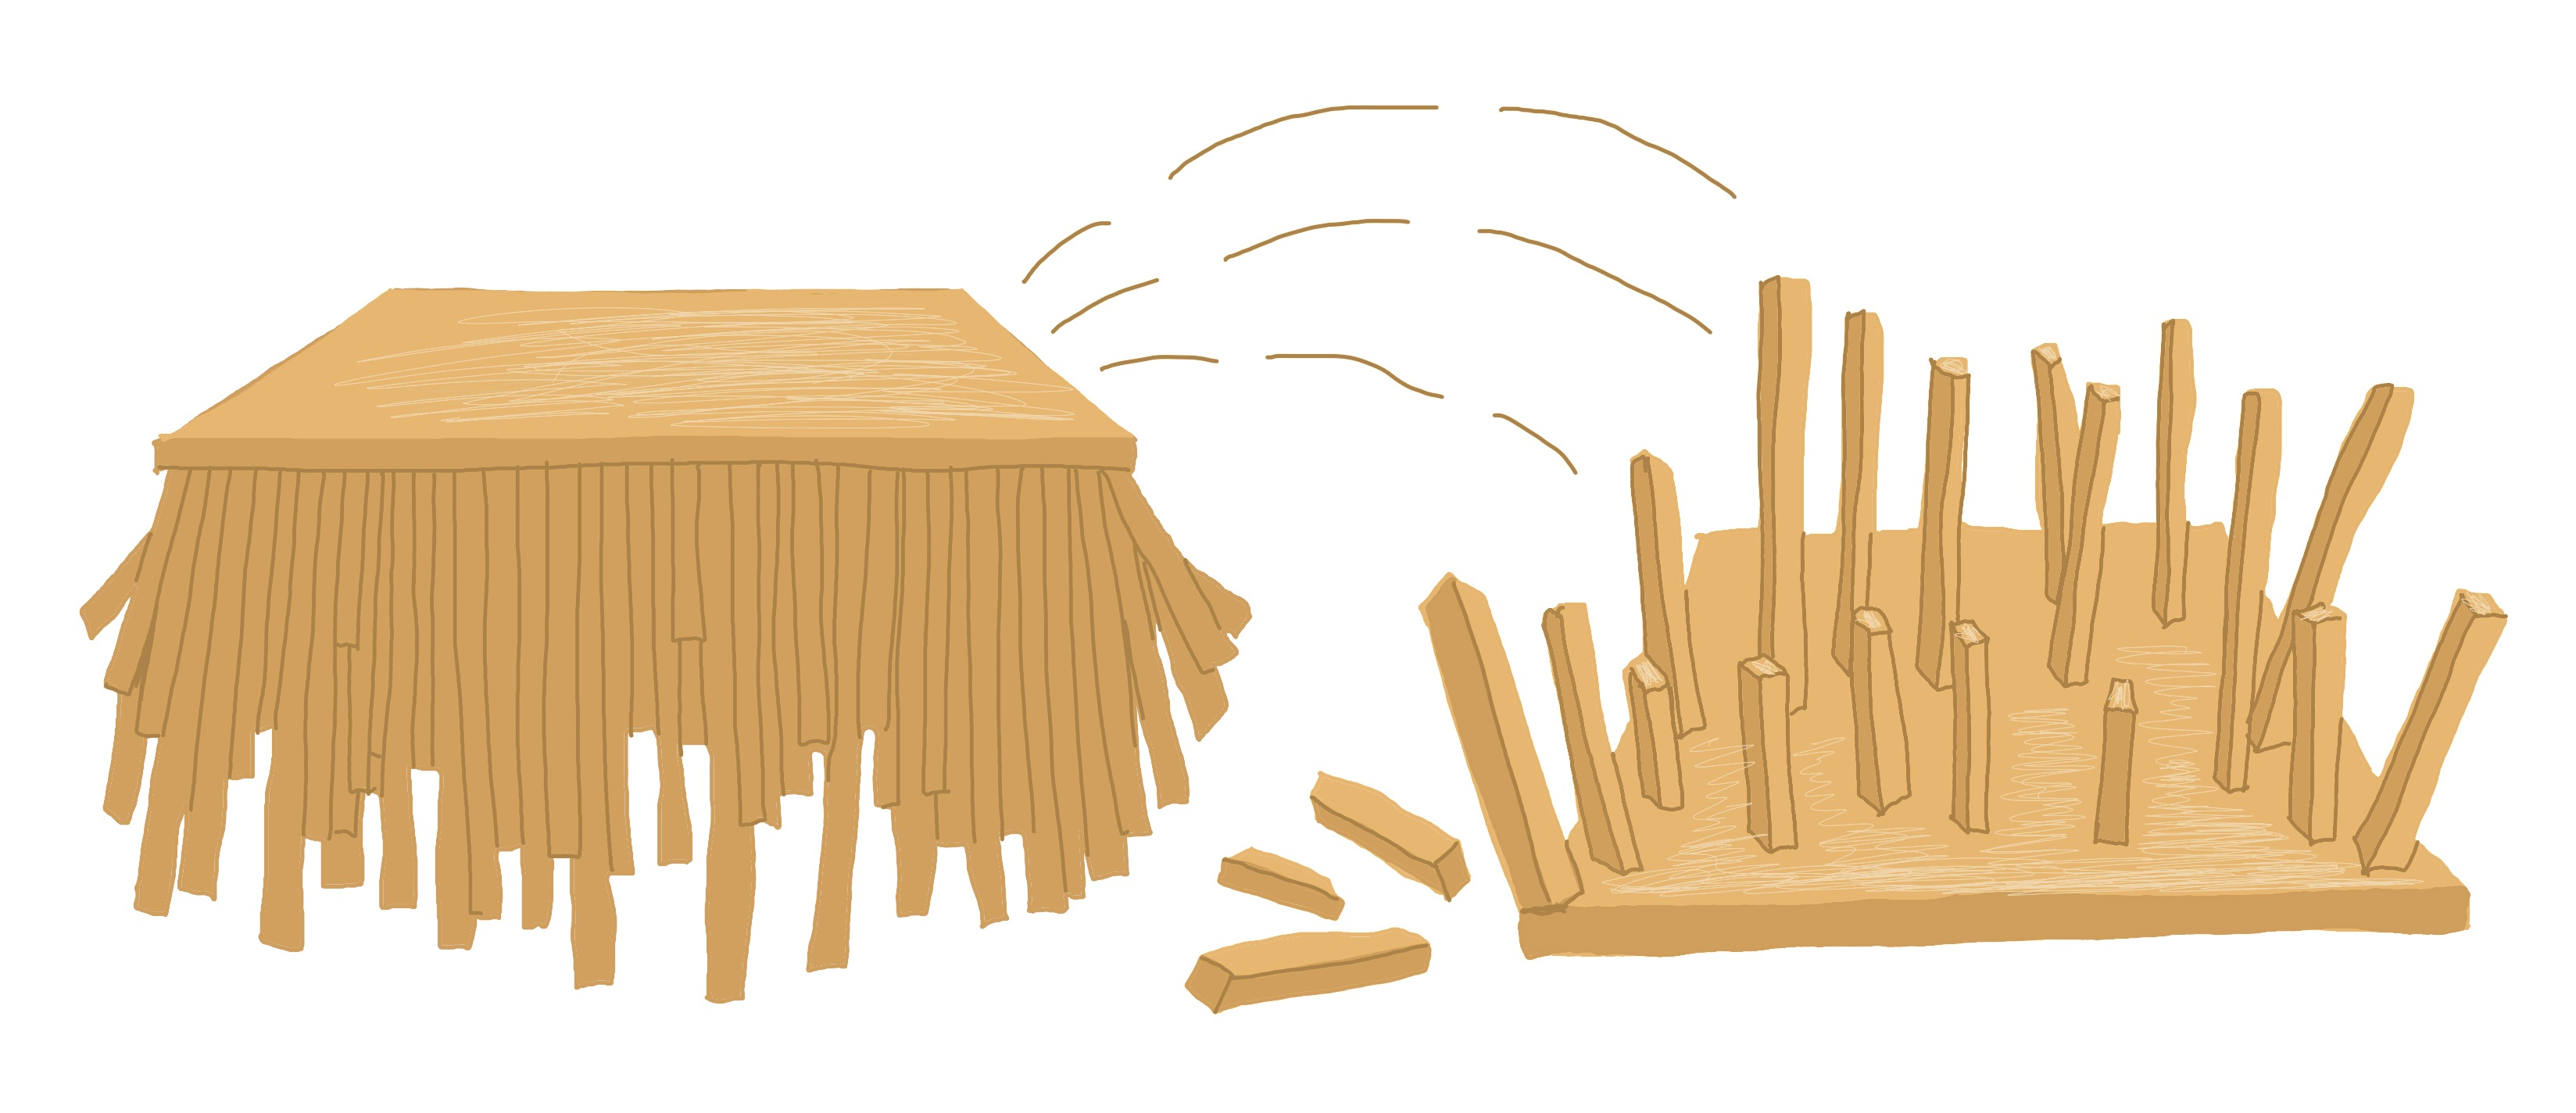
\includegraphics[width=11cm]{figures/color/01c.jpg}
	\vspace{0.5cm}
	\caption{
             {\itshape  Экспериментальный стул с использованием нанотехнологий 
             (одна из инноваций заключается, например, в том, что у 
             такого стула ровно 720 ножек) падает с лестницы }\medskip\\
             \rightline{Задача 3 <<Современная мебельная фабрика>>,}\\
             \rightline{2018 год, 5 класс}}
\end{center} \end{figure}

\begin{figure} \begin{center}
	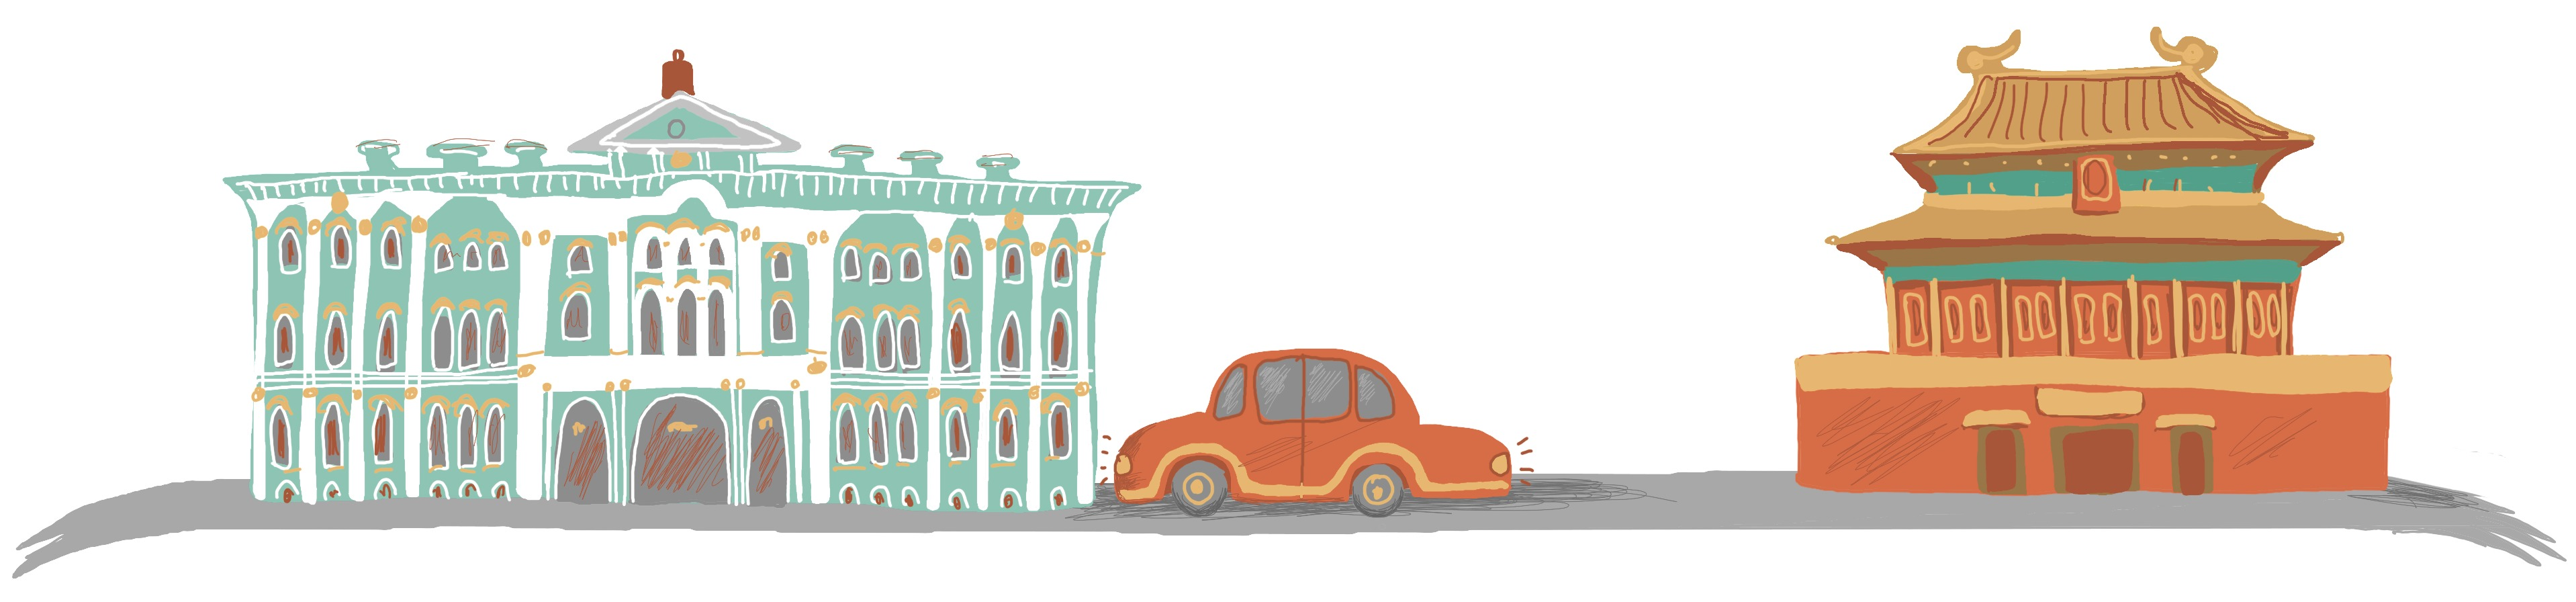
\includegraphics[width=12cm]{figures/color/15c.jpg}
	\vspace{0.5cm}
	\caption{
             {\itshape  Автомобиль выехал из Петербурга в Пекин и сломался ... %через 80 километров. 
             %На исправление неполадок ушло, правда, всего две минуты. Однако, проехав еще 40 километров, 
             %автомобиль вновь сломался, но вновь был отремонтирован за две минуты. 
             %Далее перед каждой следующей поломкой автомобиль проезжал вдвое меньше, чем перед 
             %предыдущей, но приводился в рабочее состояние за не- изменные две минуты. 
             Доедет ли он в итоге до Пекина? }\medskip\\
             \rightline{Задача 2 <<Шутка>>, 2017 год, 5 класс}}
\end{center} \end{figure}


\begin{figure} \begin{center}
	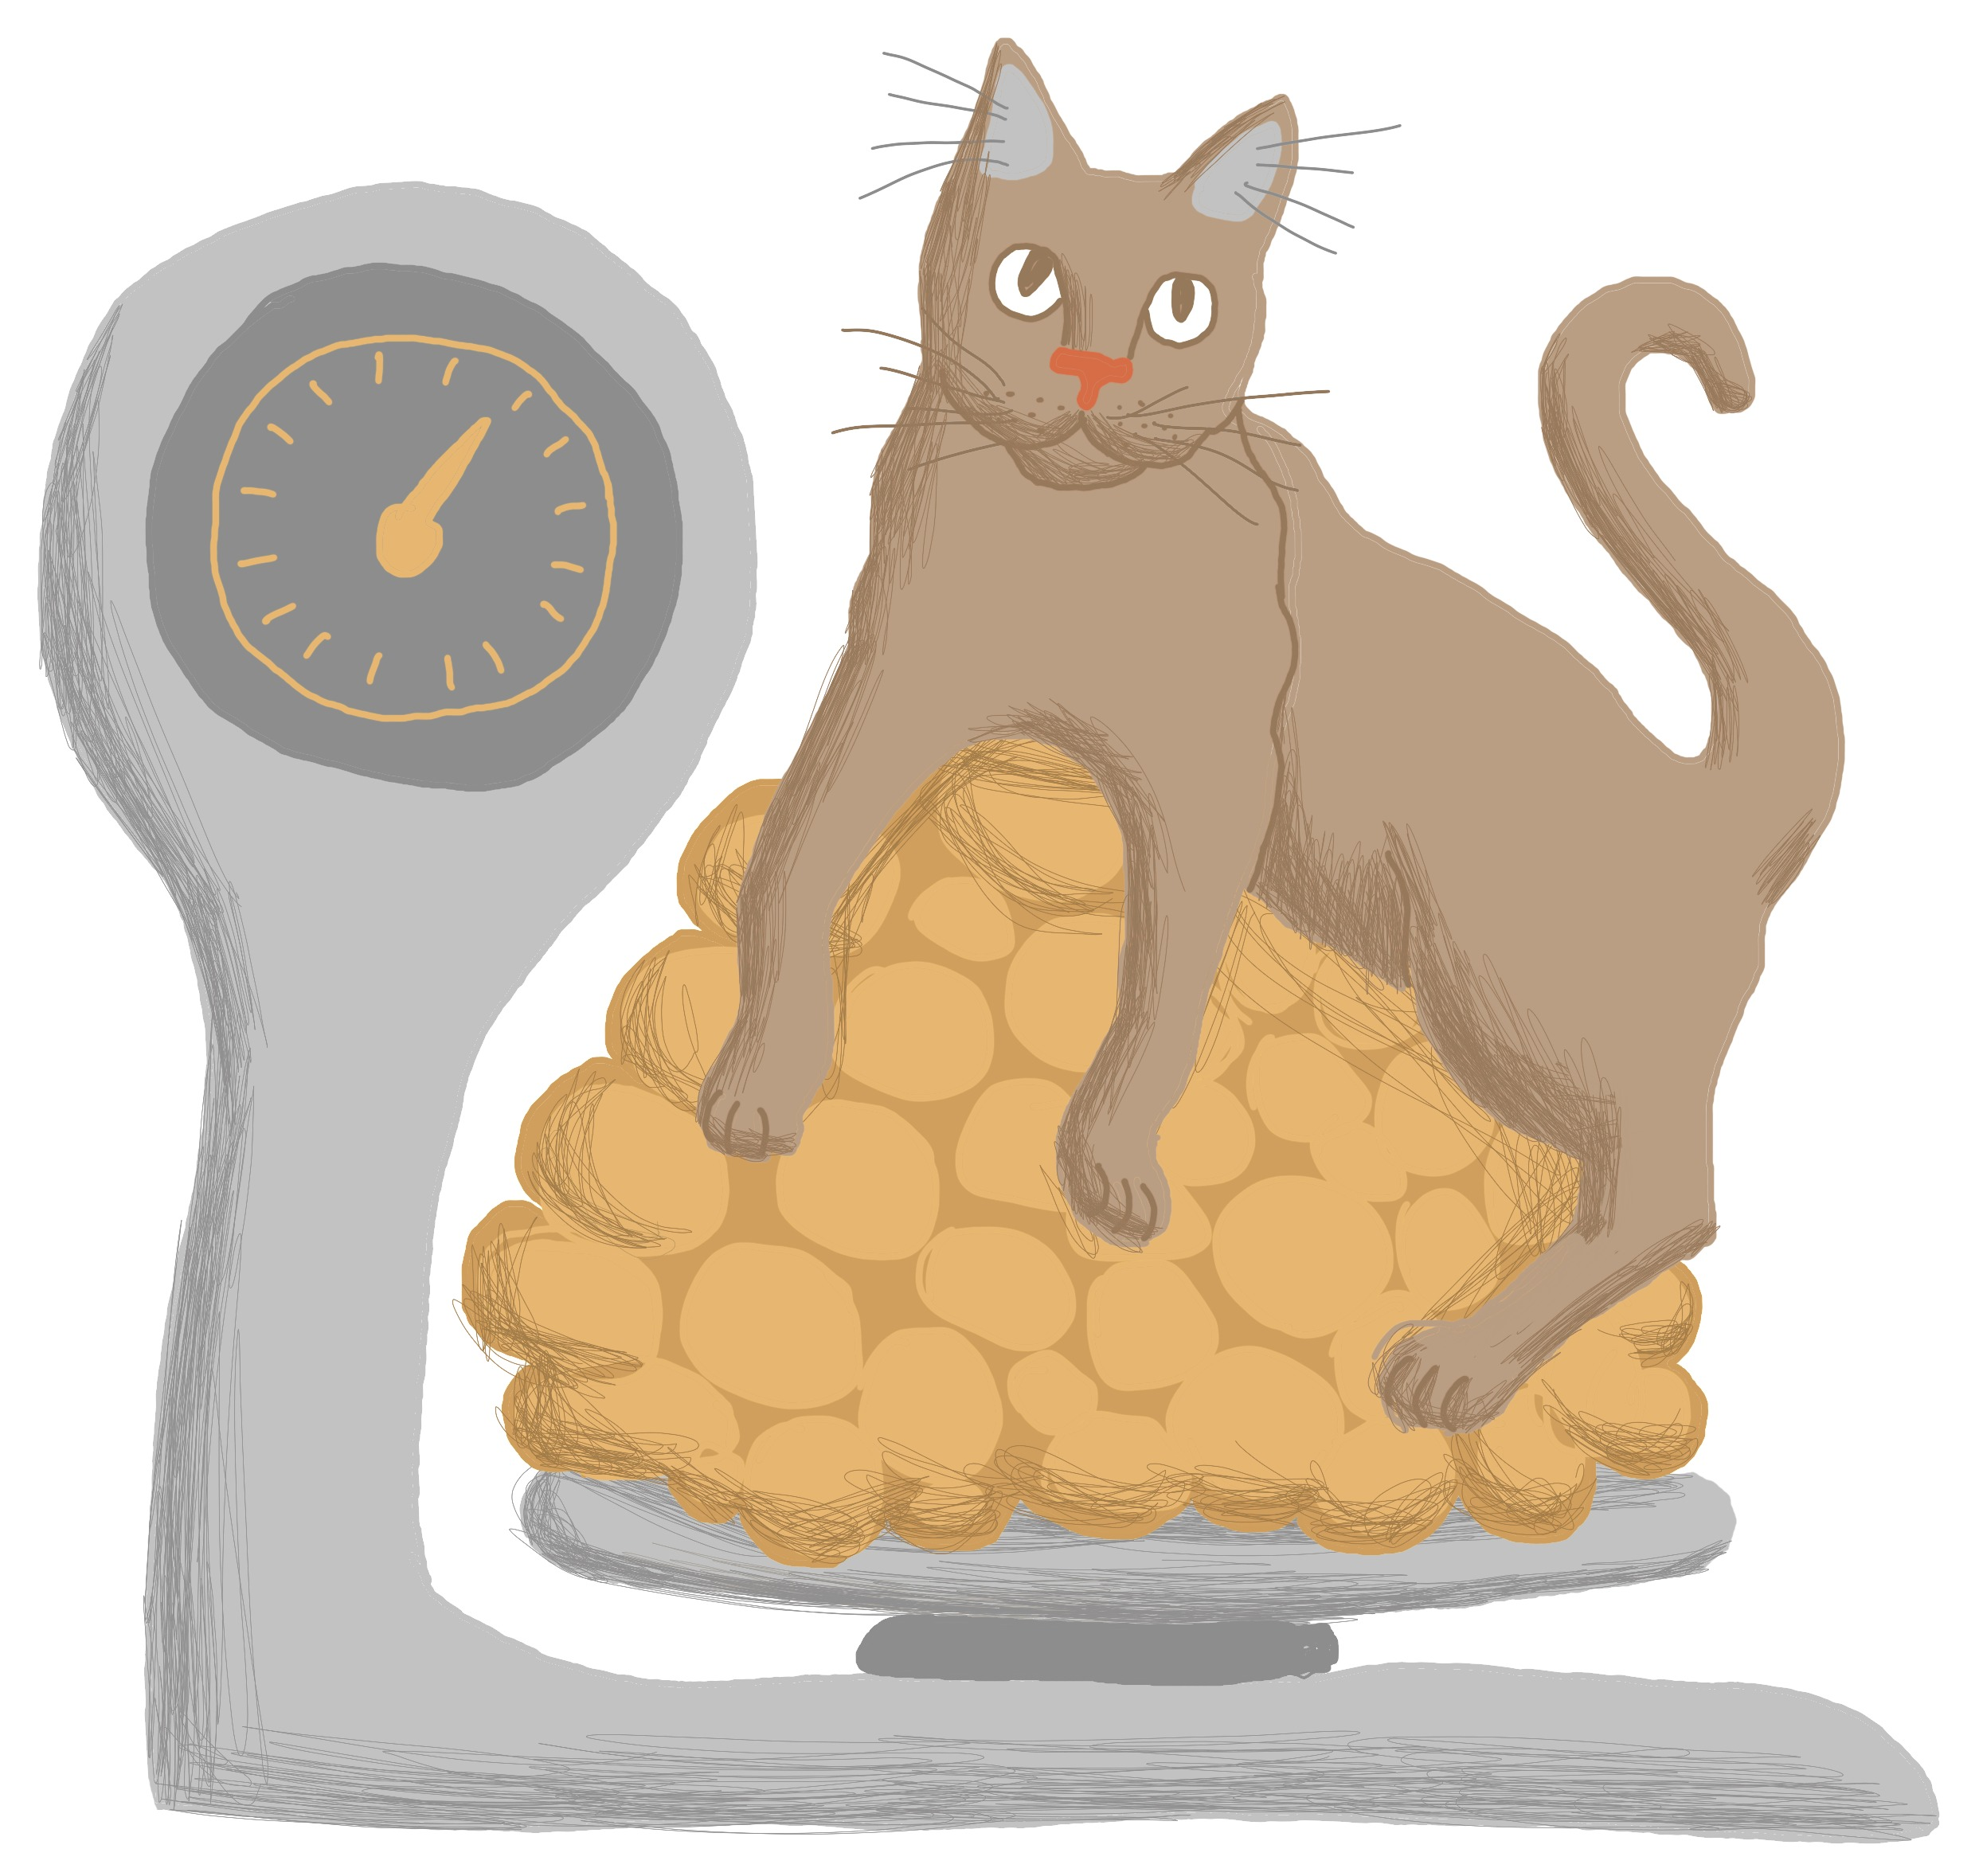
\includegraphics[width=10cm]{figures/color/02c.jpg}
	\vspace{1cm}
	\caption{
             {\itshape  При взвешивании картофеля получилось 1000 граммов, при 
             взвешивании домашнего кота — 4400 граммов. При взвешивании кота вместе 
             с картофелем --- 5000 граммов. Чему же равна погрешность весов? }\medskip\\
             \rightline{Задача 7 <<Взвешивания>>, 2017 год, 7 класс}}
\end{center} \end{figure}

\begin{figure} \begin{center}
	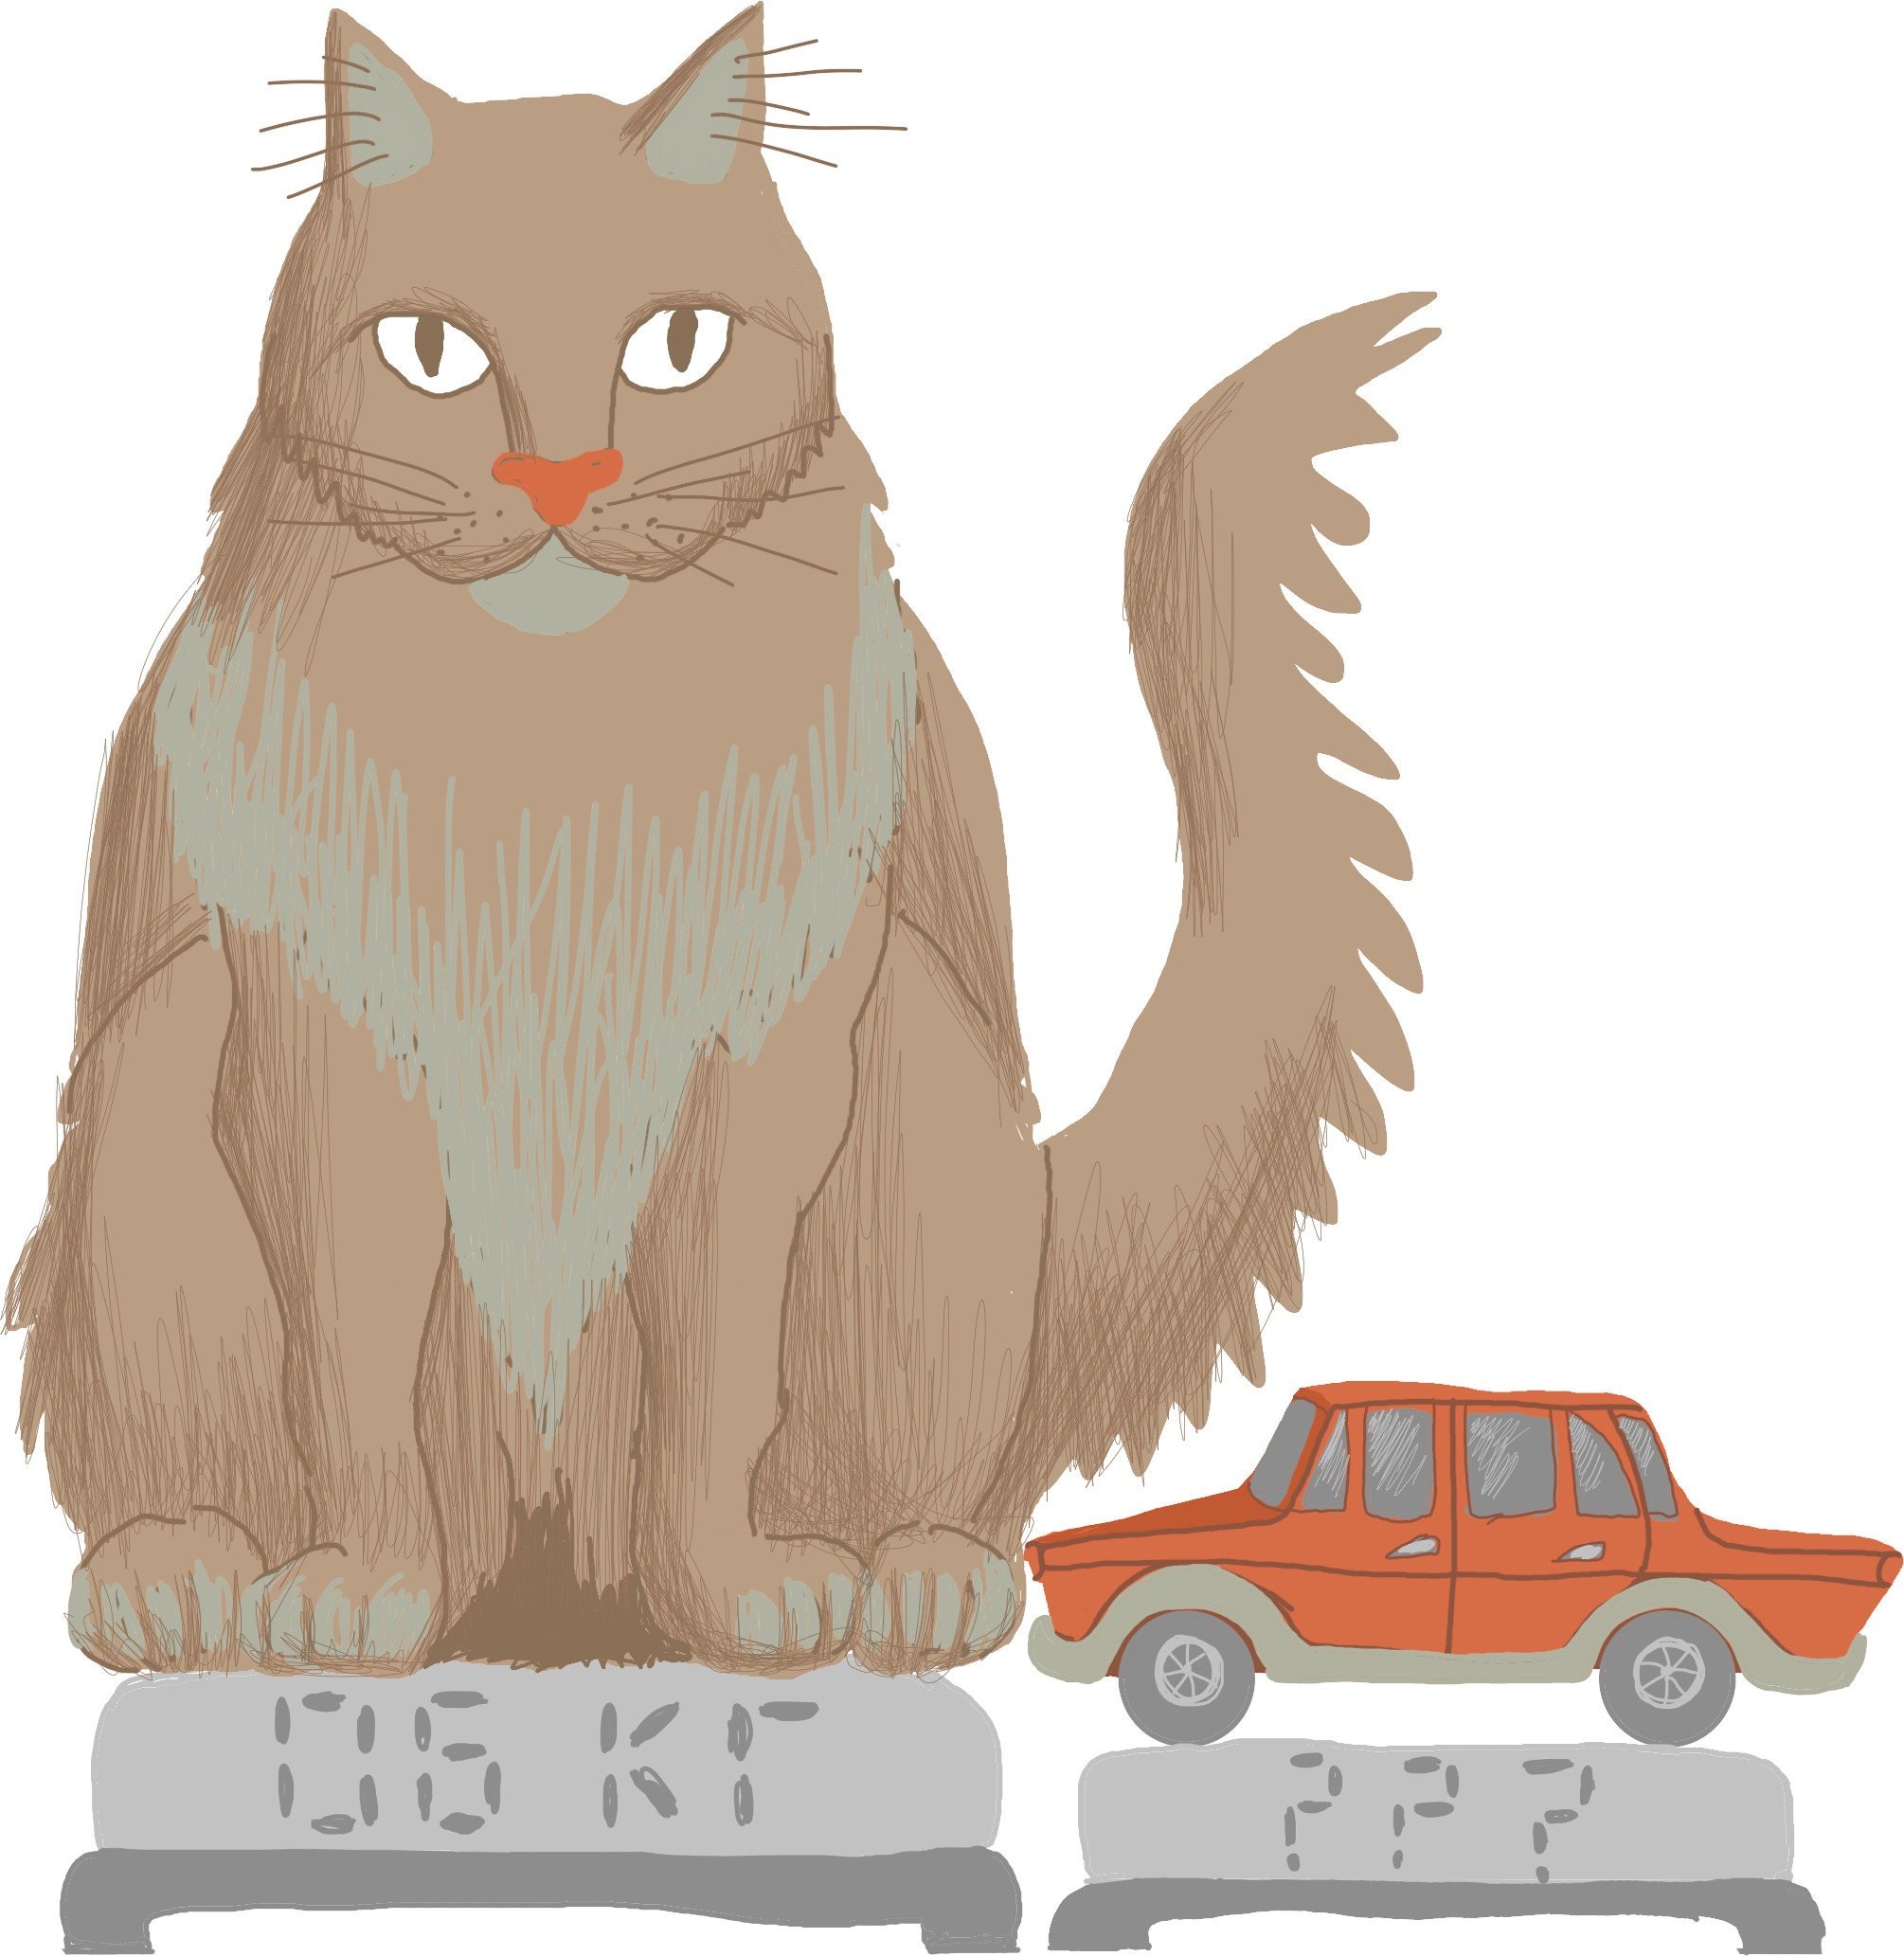
\includegraphics[width=10cm]{figures/color/03c.jpg}
	\vspace{1cm}
	\caption{
             {\itshape  Моделька должна весить $1200 / 43 \approx 28$ килограммов... 
             Однако она ощутимо легче моего кота, про которого мама недавно сказала, 
             что он толстый, потому что преодолел отметку в 6 кило. Где же логика? }\medskip\\
             \rightline{Задача 4 <<Модельки>>, 2018 год, 6 класс}}
\end{center} \end{figure}

\begin{figure} \begin{center}
	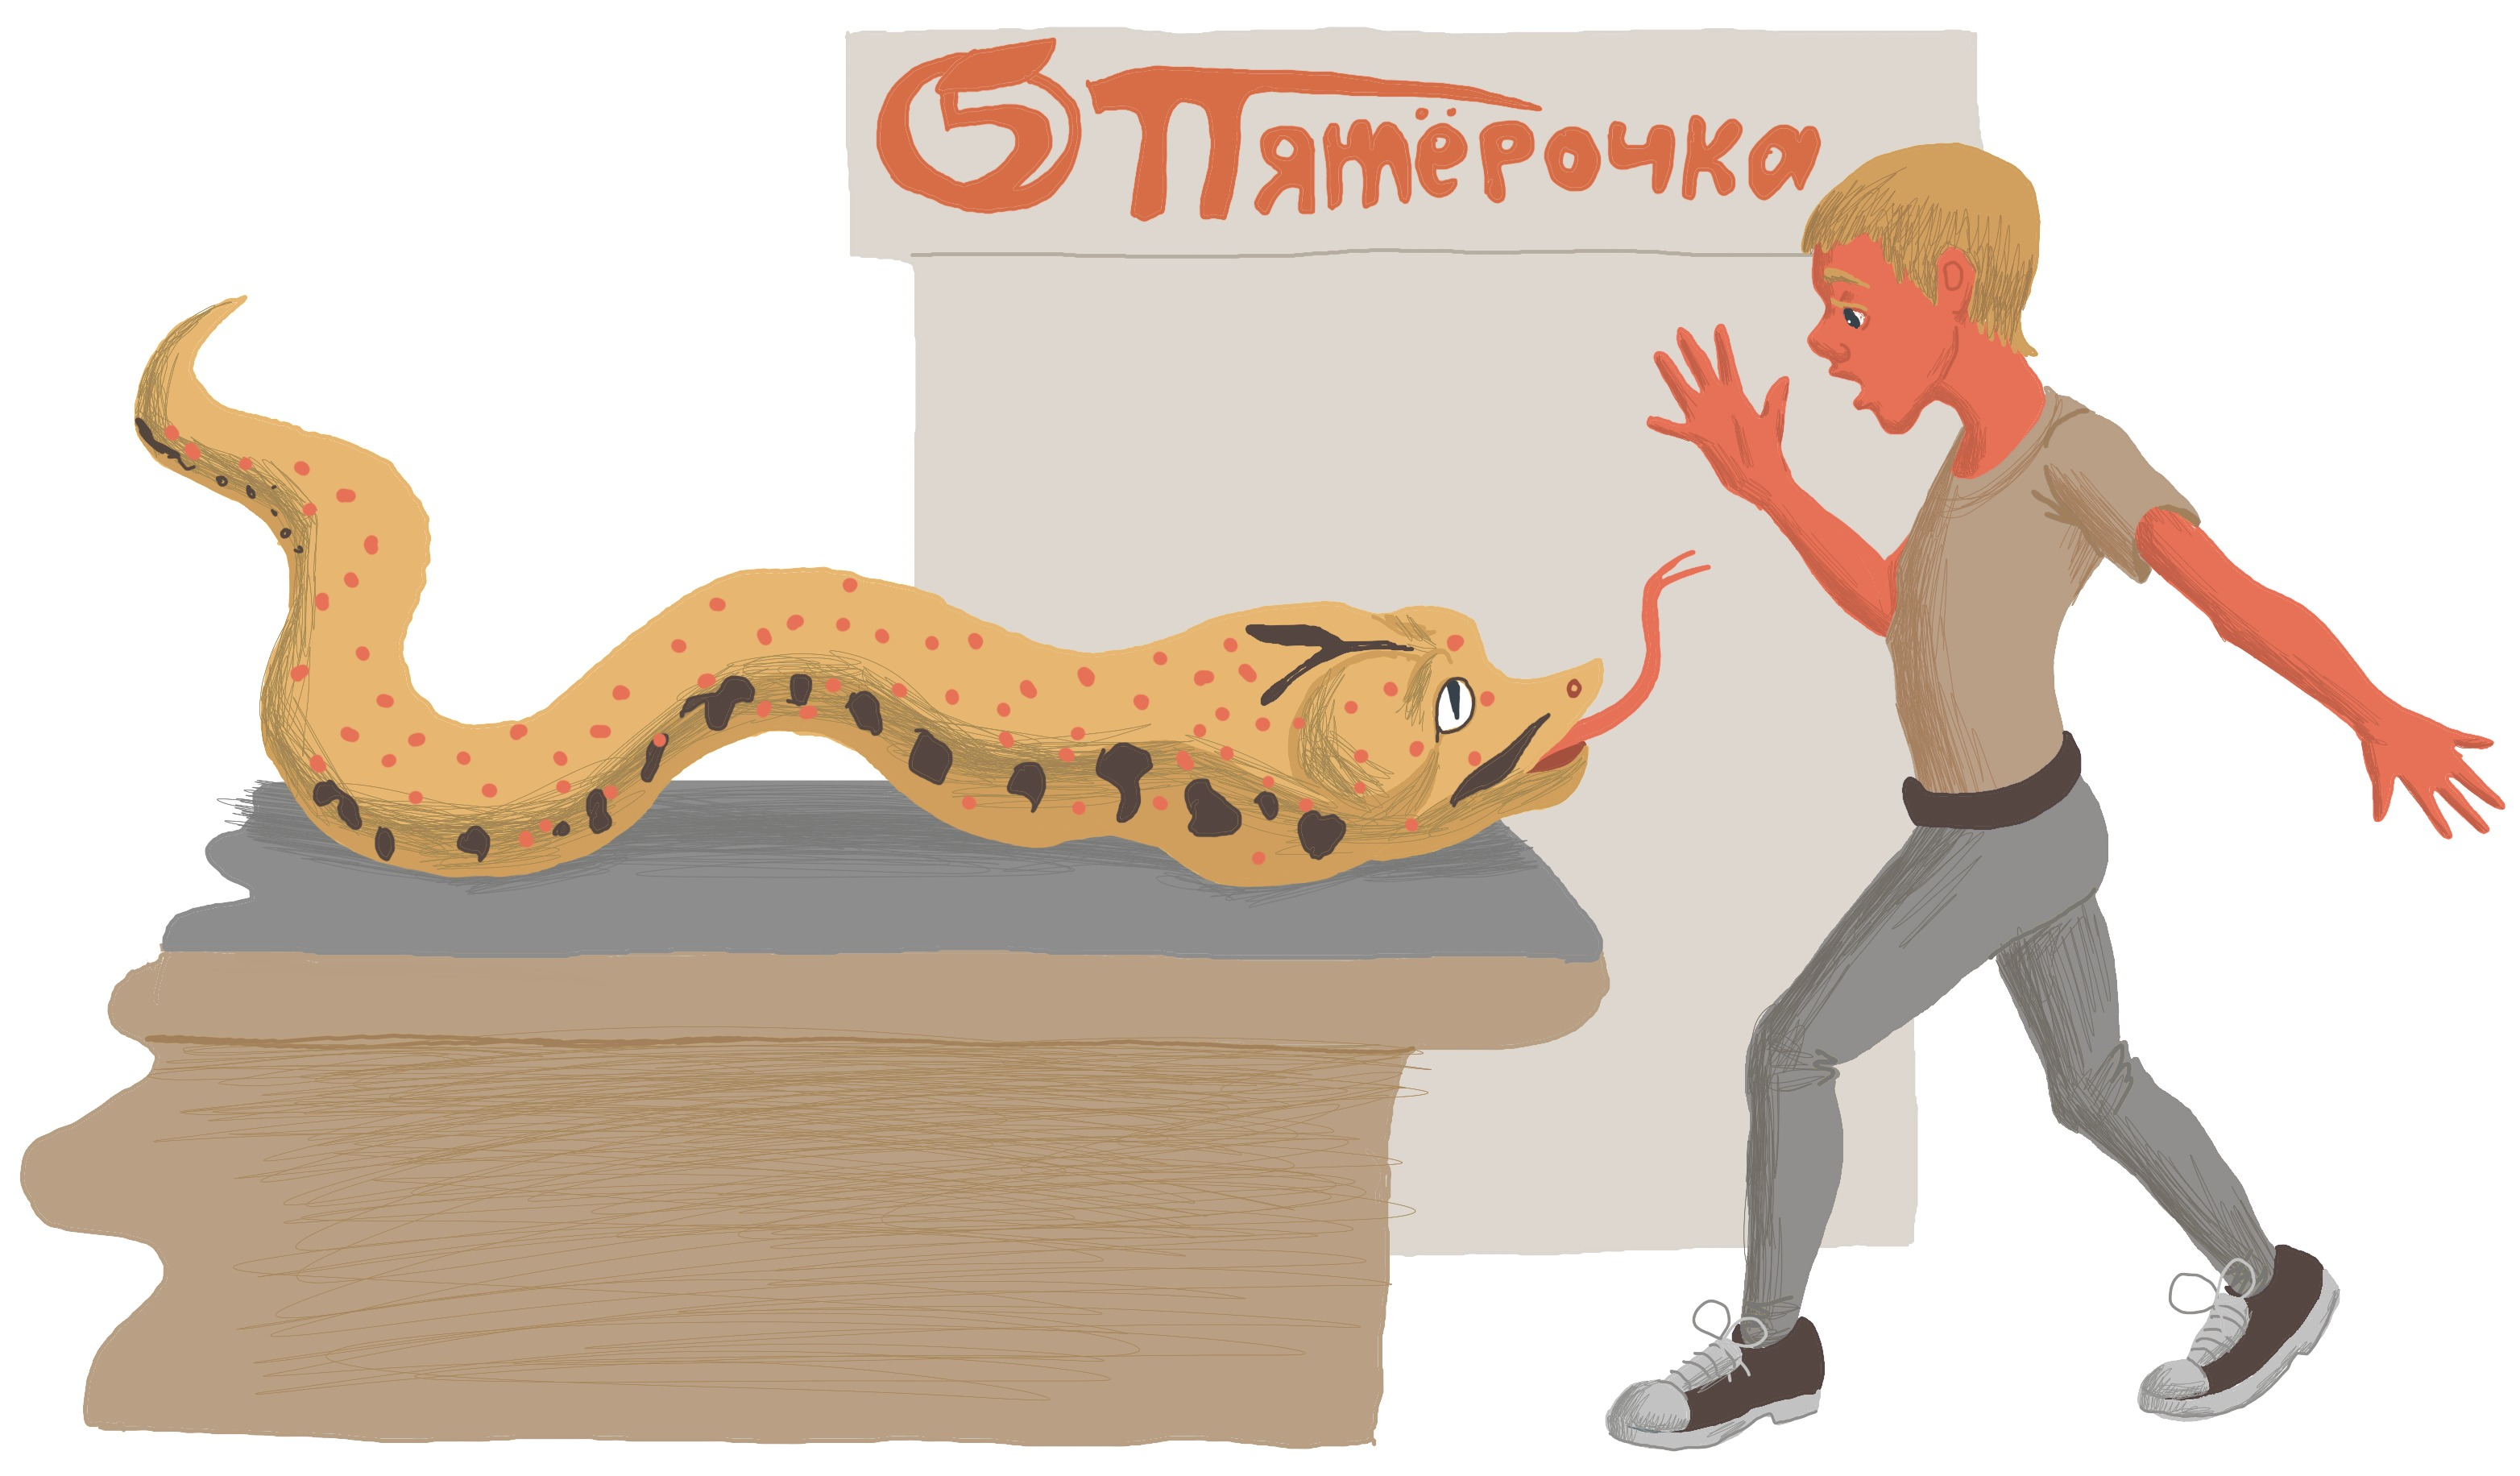
\includegraphics[width=11cm]{figures/color/04c.jpg}
	\vspace{1cm}
	\caption{
             {\itshape  Если транспортер движется со скоростью $v$ м/с, то лежащий 
             на нем питон проезжает мимо неподвижного наблюдателя за 14 секунд. 
             Давайте возьмем питона–детеныша (его длина составляет $\tfrac{3}{4}$ от 
             длины взрослого питона)... %, в шесть раз более медленный транспортер, а также 
             %заставим наблюдателя идти со скоростью $\tfrac{1}{3}v$~м/с навстречу транспортеру. 
             За какое время детеныш питона пронесется мимо наблюдателя? }\medskip\\
             \rightline{Задача 6 <<Как провожают транспортеры...>>}\\
             \rightline{2018 год, 7 класс}}
\end{center} \end{figure}

\vfill\eject

\begin{figure} \begin{center}
	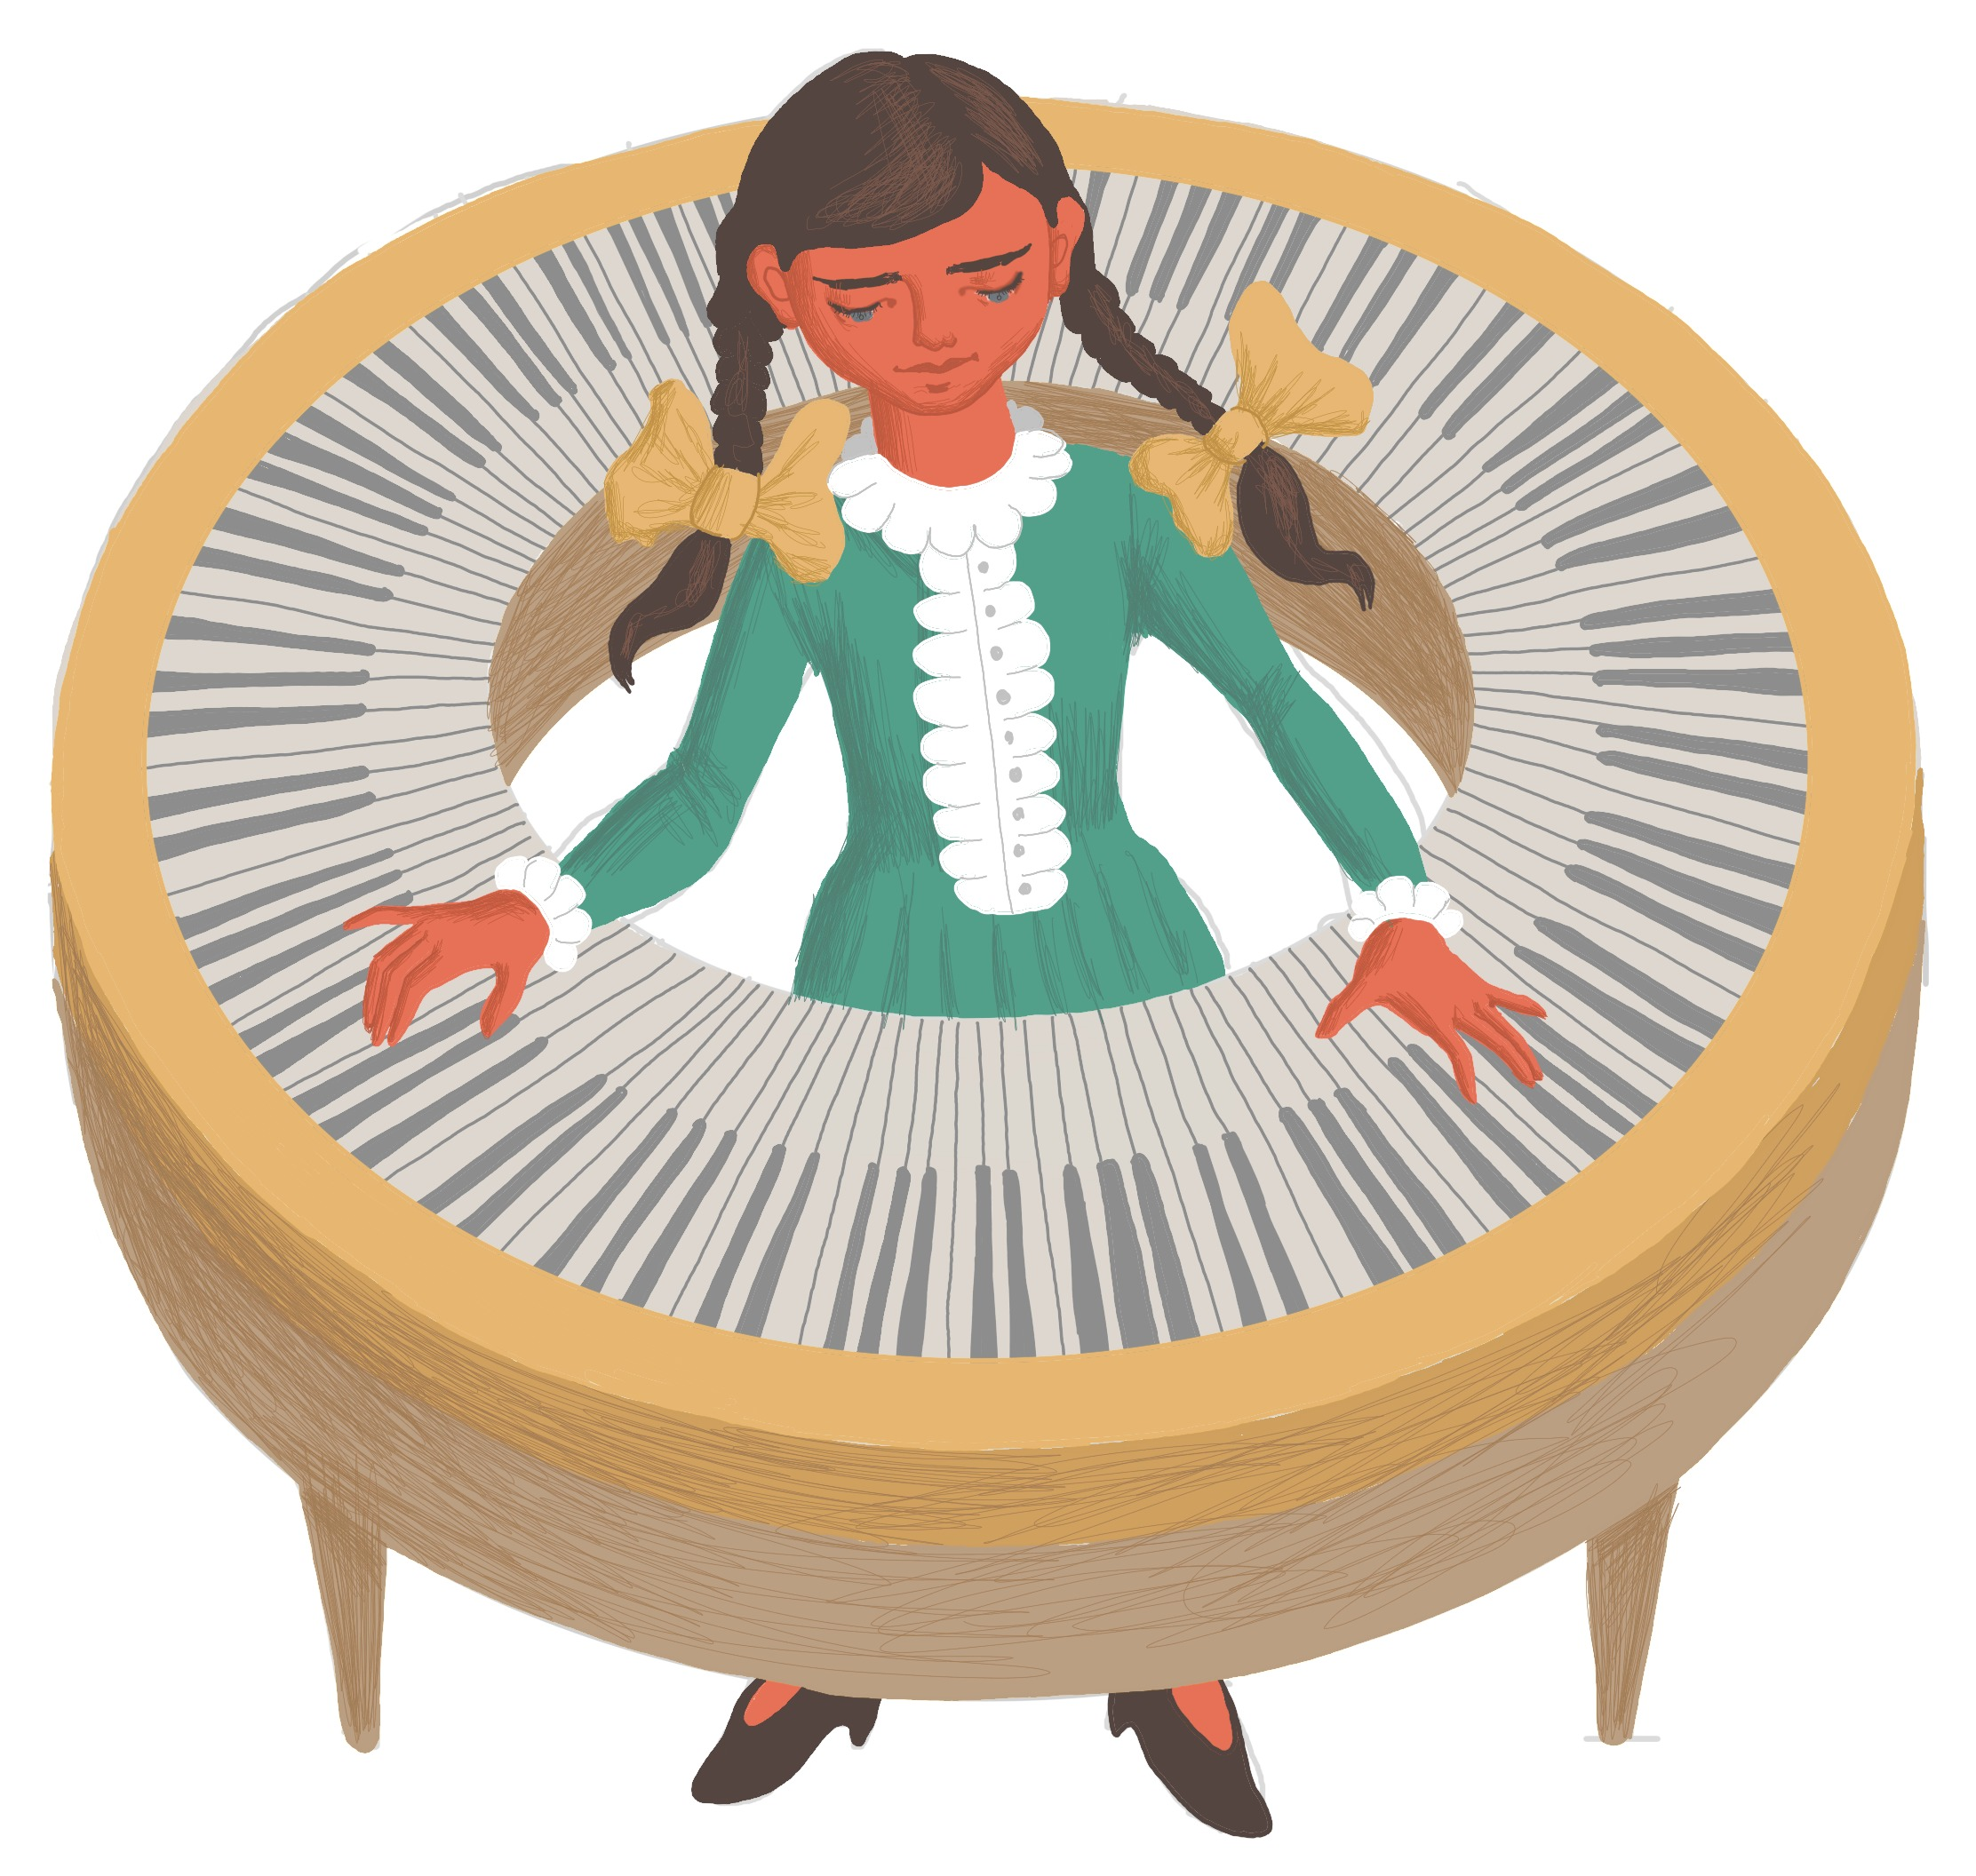
\includegraphics[width=10cm]{figures/color/06c.jpg}
	\vspace{1cm}
	\caption{
             {\itshape  Девочка Лина играет на круговом фортепиано аналог 
              «Лунной сонаты» собственного сочинения }\medskip\\
             \rightline{Задача 6 <<И пусть Бетховен услышит>>}\\
             \rightline{2017 год, 5 класс}}
\end{center} \end{figure}

\begin{figure} \begin{center}
	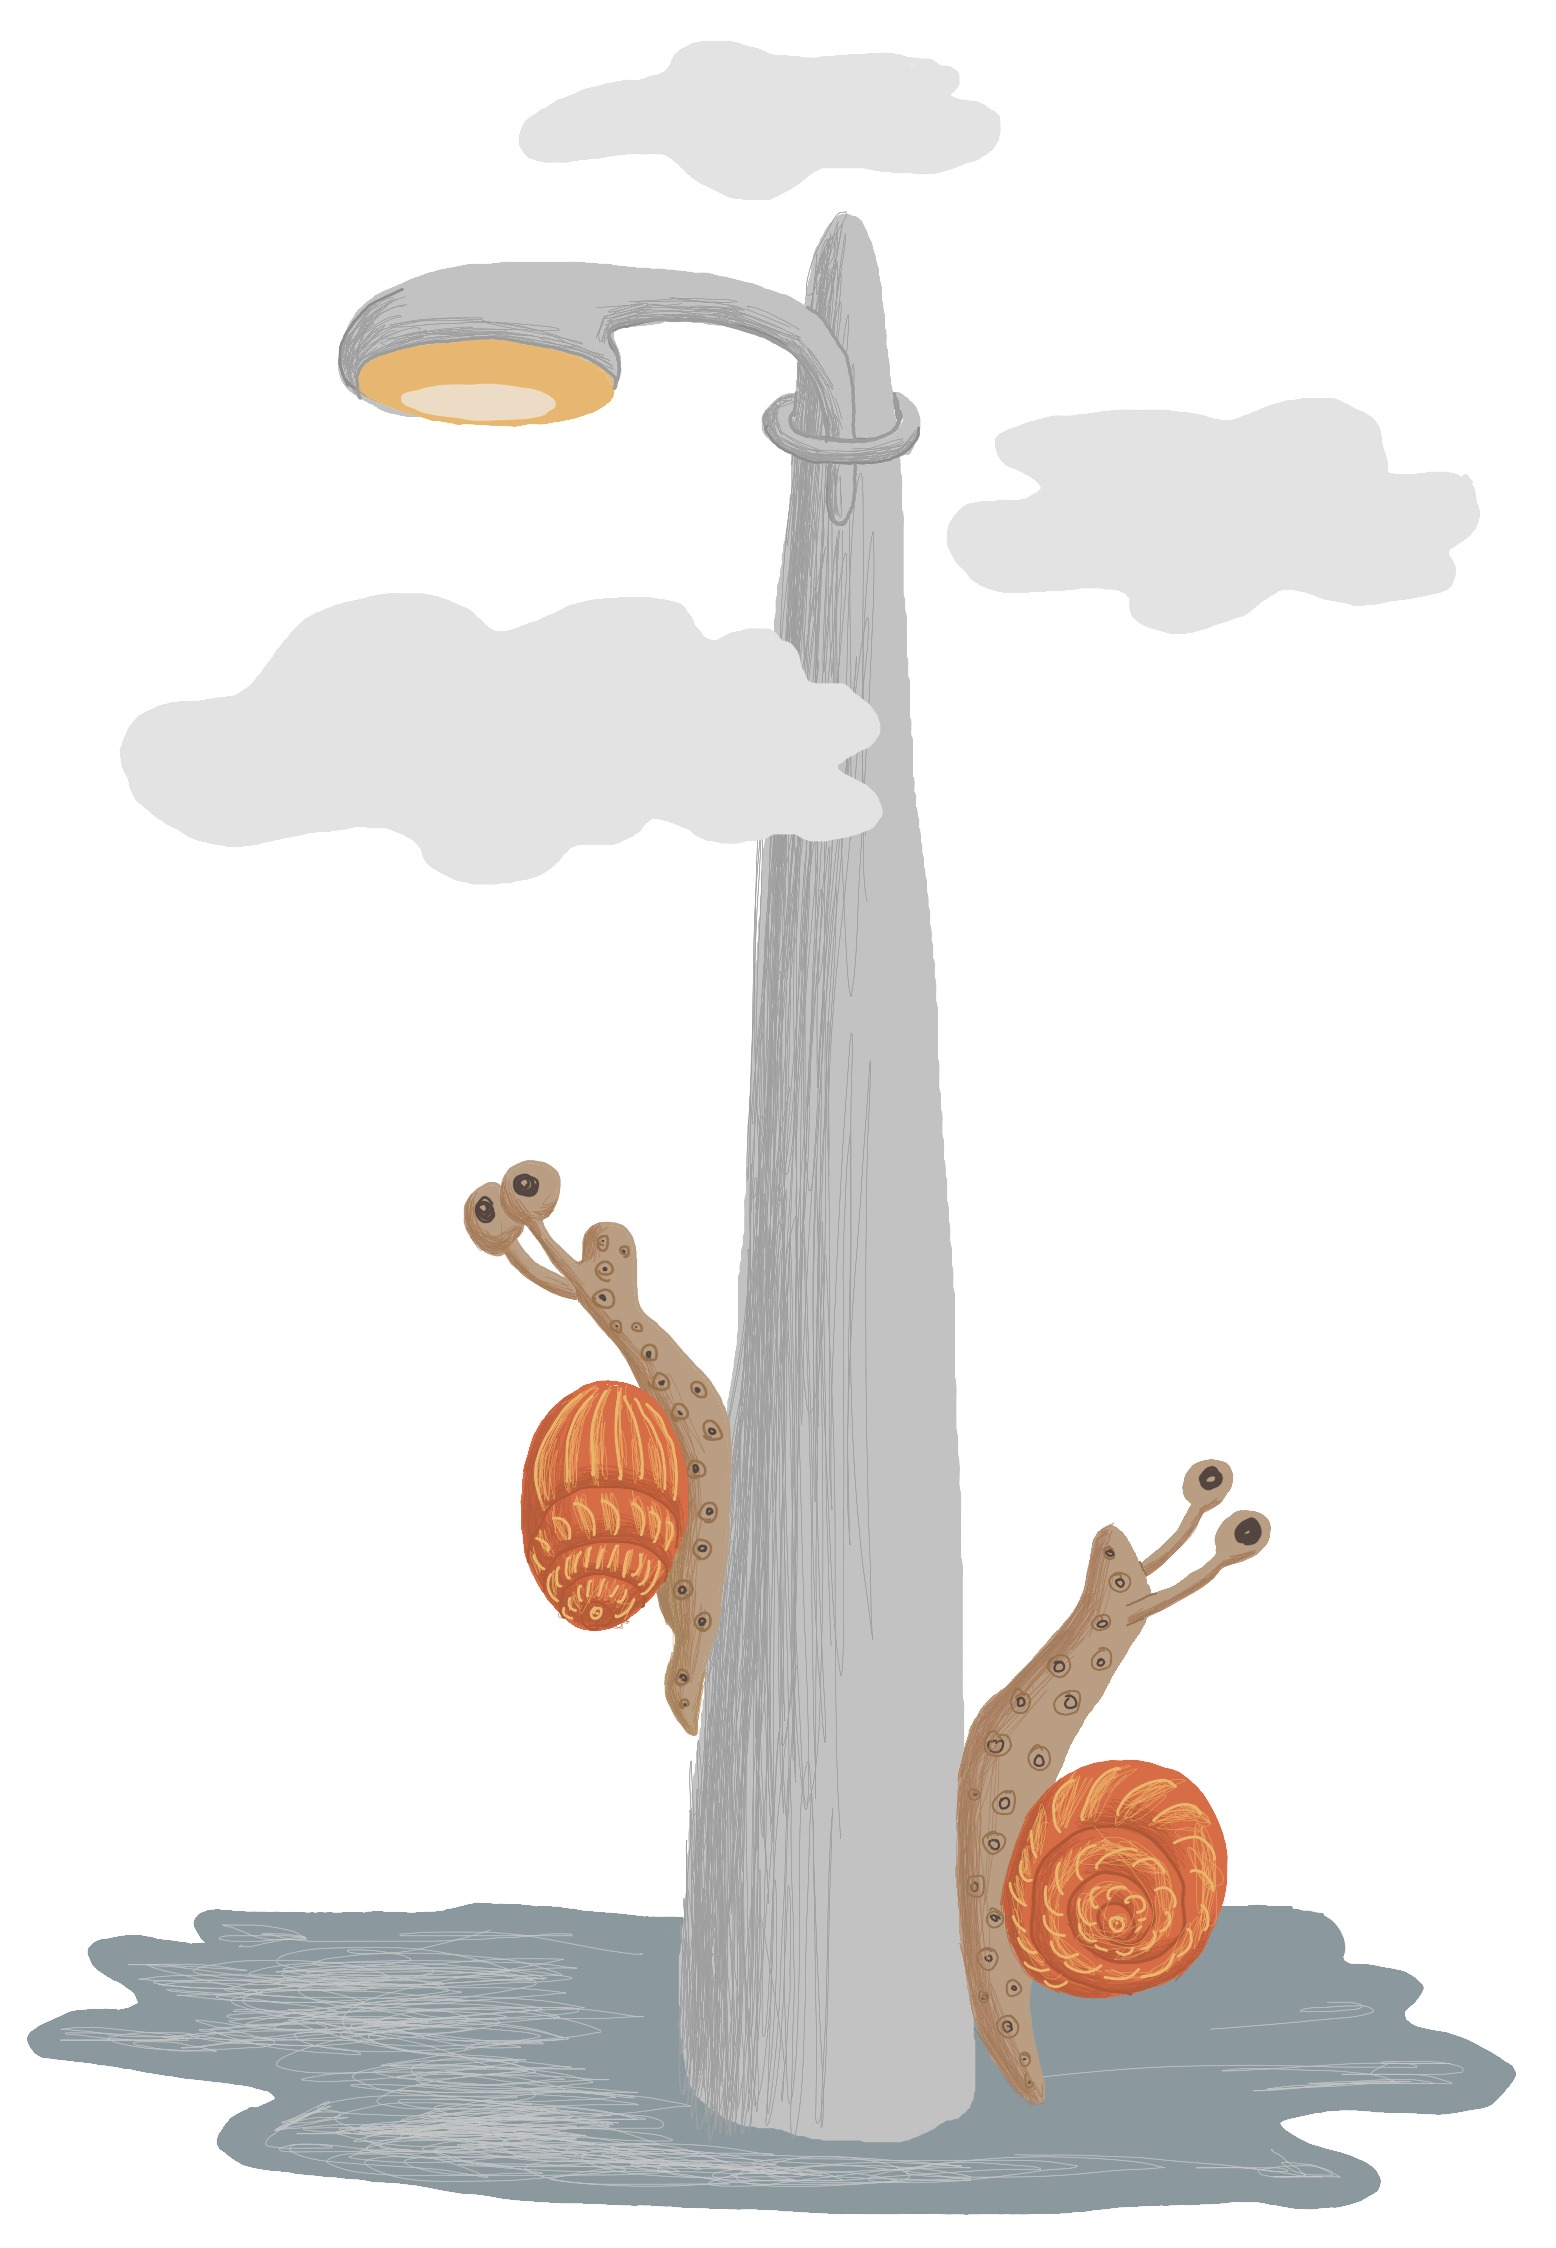
\includegraphics[width=8cm]{figures/color/07c.jpg}
	\vspace{1cm}
	\caption{
             {\itshape  Две улитки ползут снизу вверх по столбу высотой 7 метров }\medskip\\
             \rightline{Задача 2 <<Гонки улиток>>, 2017 год, 7 класс}}
\end{center} \end{figure}

\begin{figure} \begin{center}
	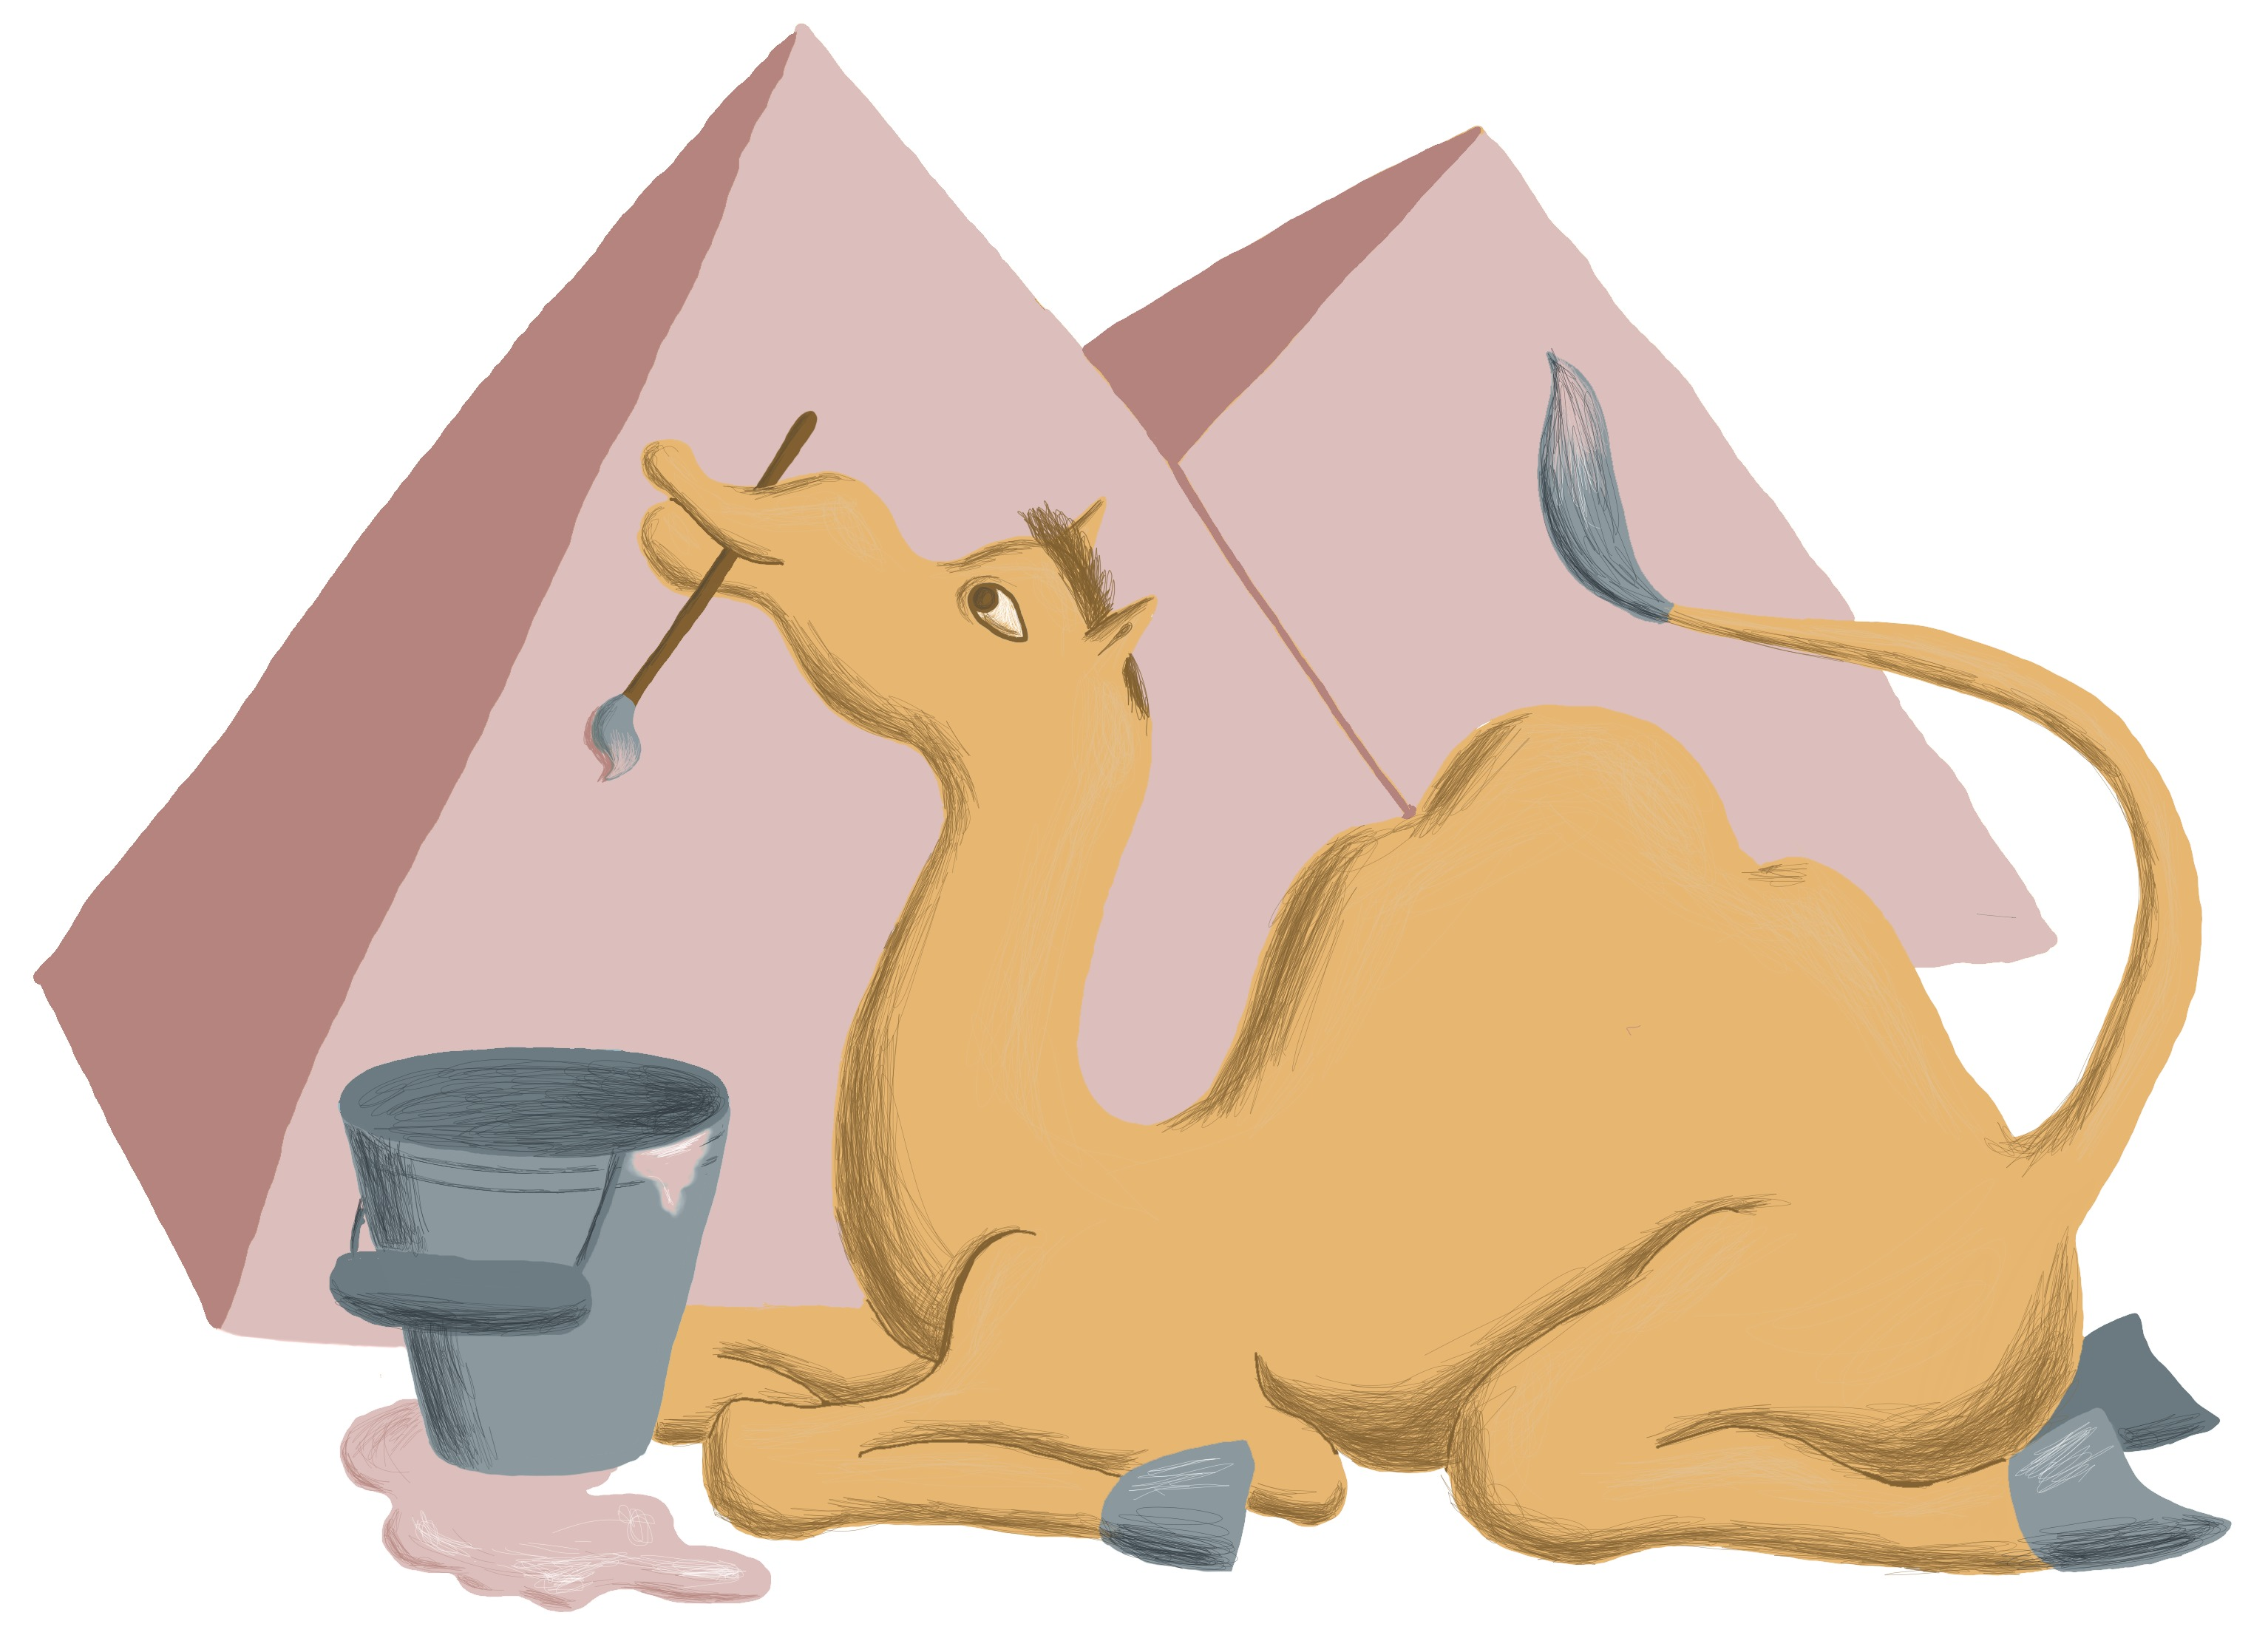
\includegraphics[width=8cm]{figures/color/19c.jpg}
	\vspace{0.5cm}
	\caption{
             {\itshape  Представьте, что одну из египетских пирамид 
             (египетские пирамиды симметричны и имеют в основании квадрат) 
             покрасили розовой краской }\medskip\\
             \rightline{Задача 3 <<Разрезания>>, 2018 год, 4 класс}}
\end{center} \end{figure}

\begin{figure} \begin{center}
	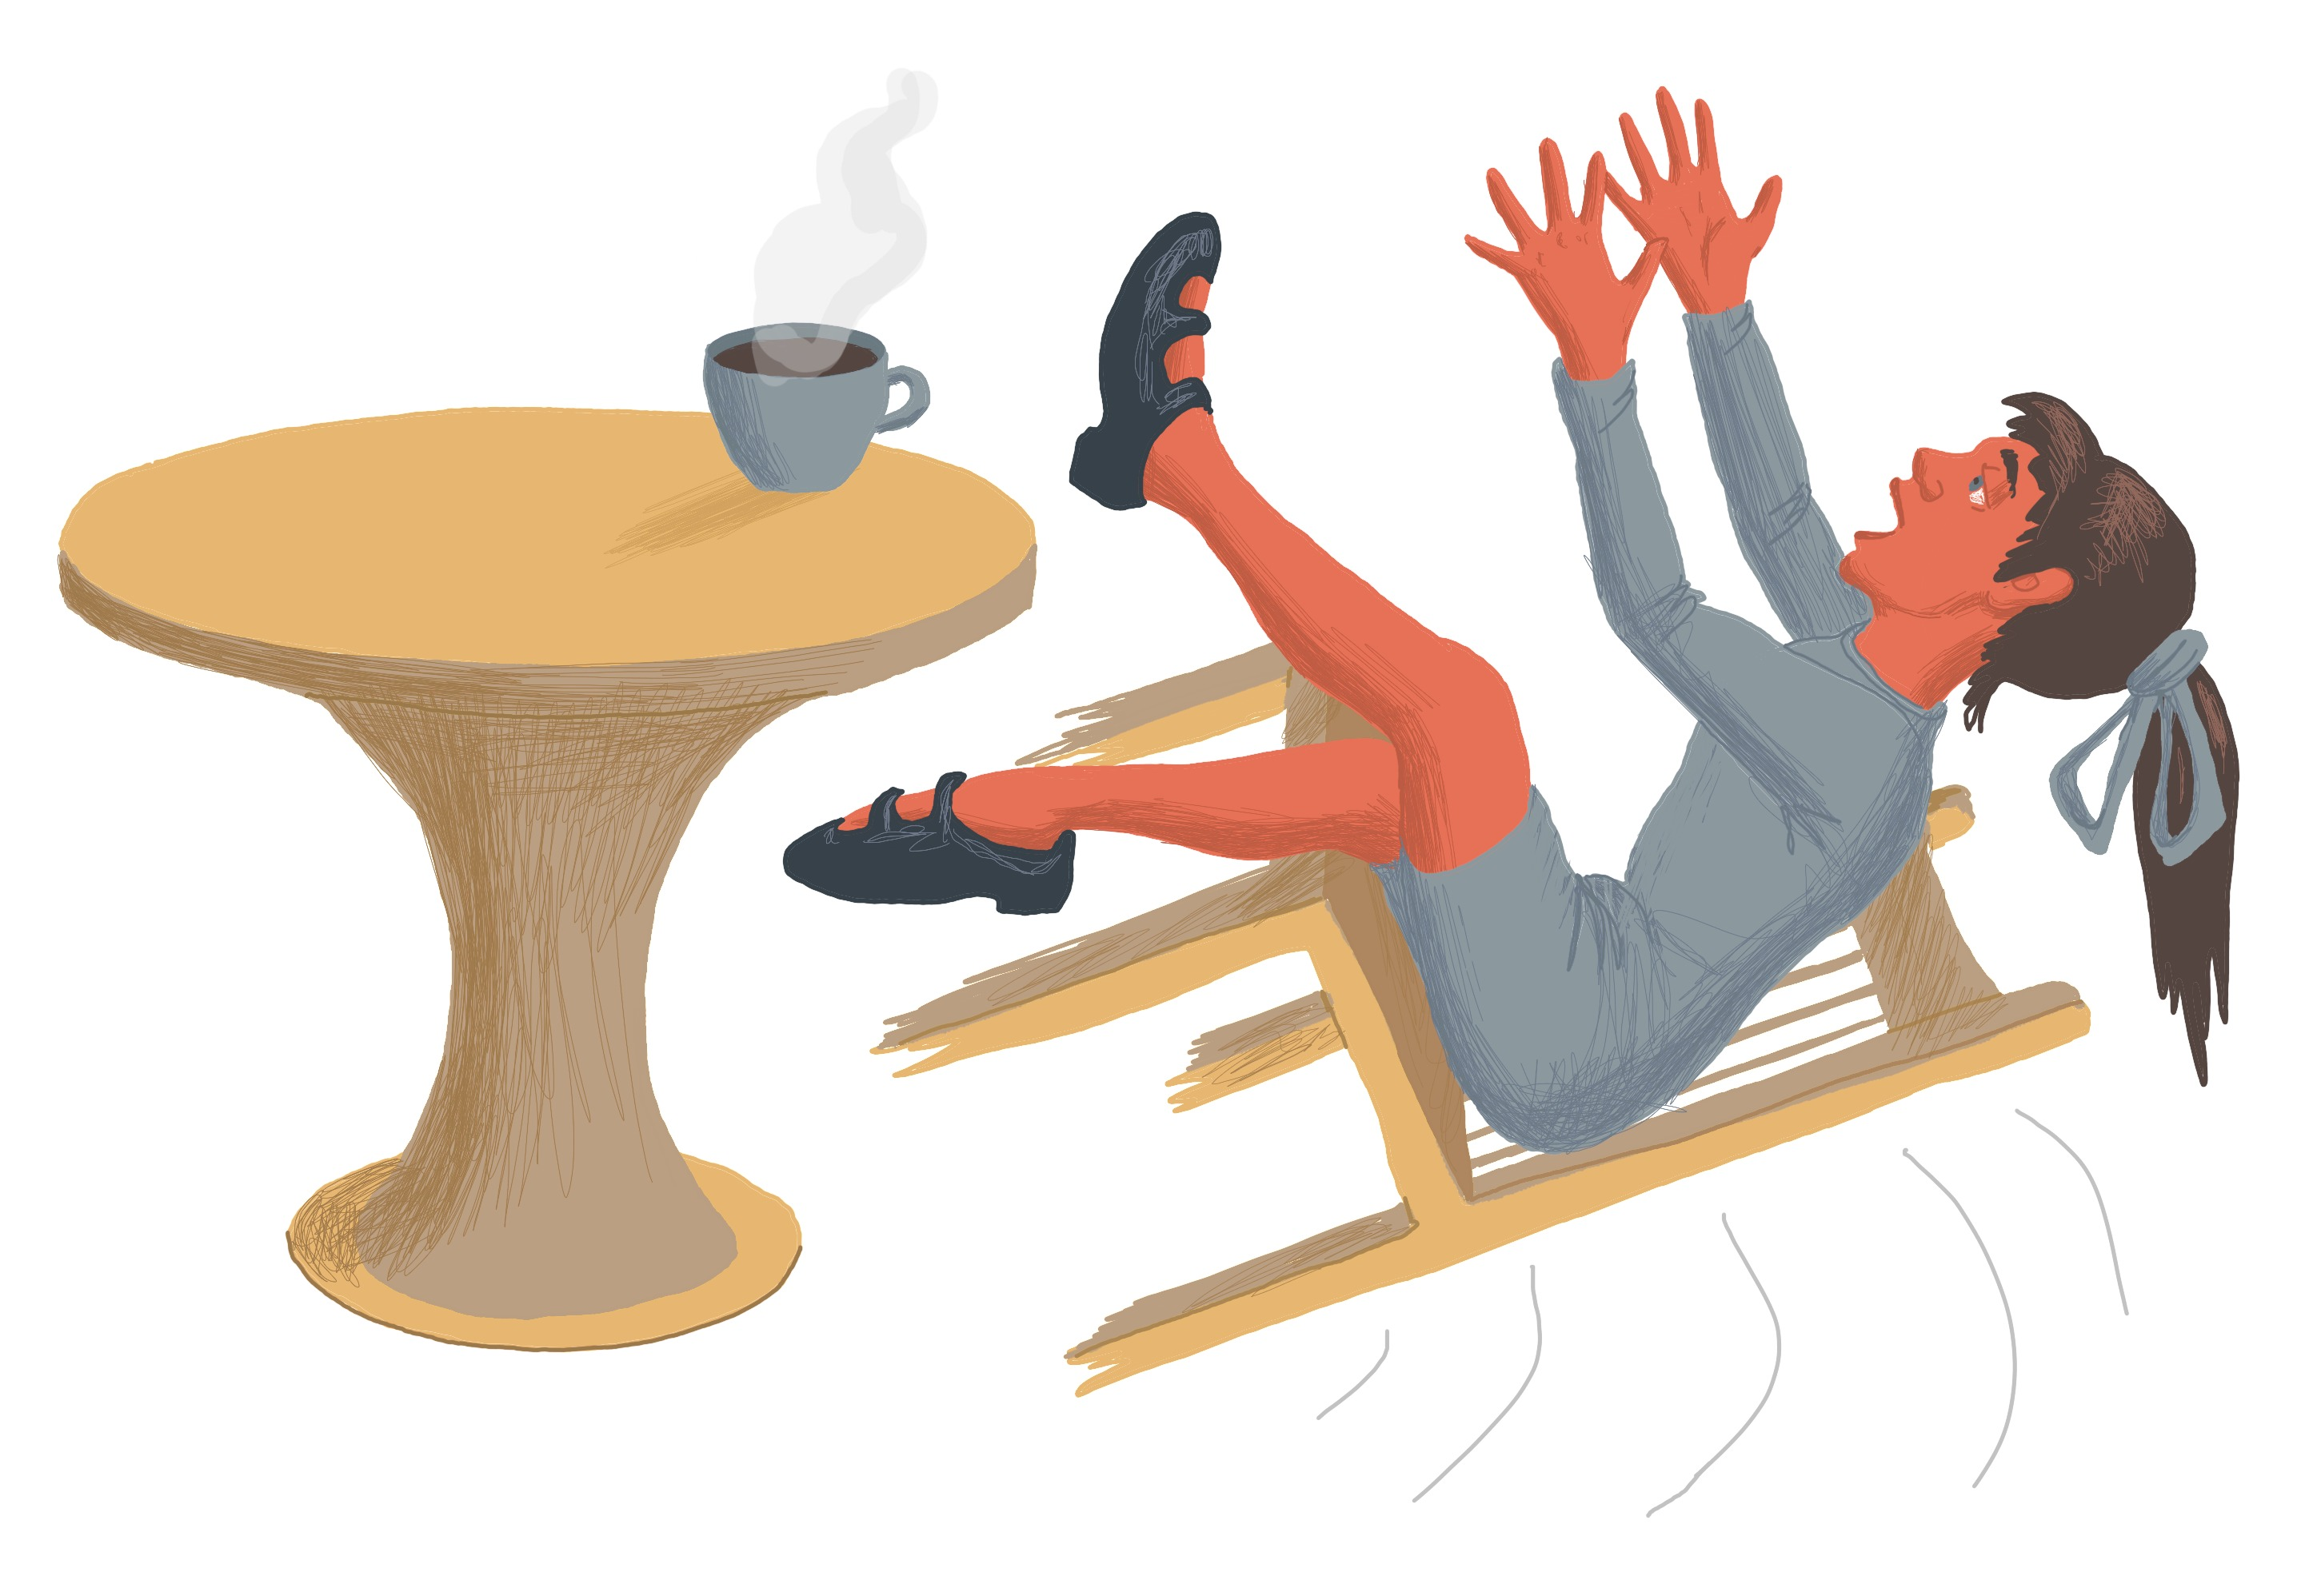
\includegraphics[width=8cm]{figures/color/05c.jpg}
	\vspace{0.2cm}
	\caption{
             {\itshape  Сколько ножек нужно подпилить Васе, 
              чтобы с утра как минимум $\mathrm{m}$ посетителей кафе гарантированно упали? }\medskip\\
             \rightline{Задача 1 <<Падающие стулья>>, 2016 год, 6 класс}}
\end{center} \end{figure}


\begin{figure} \begin{center}
	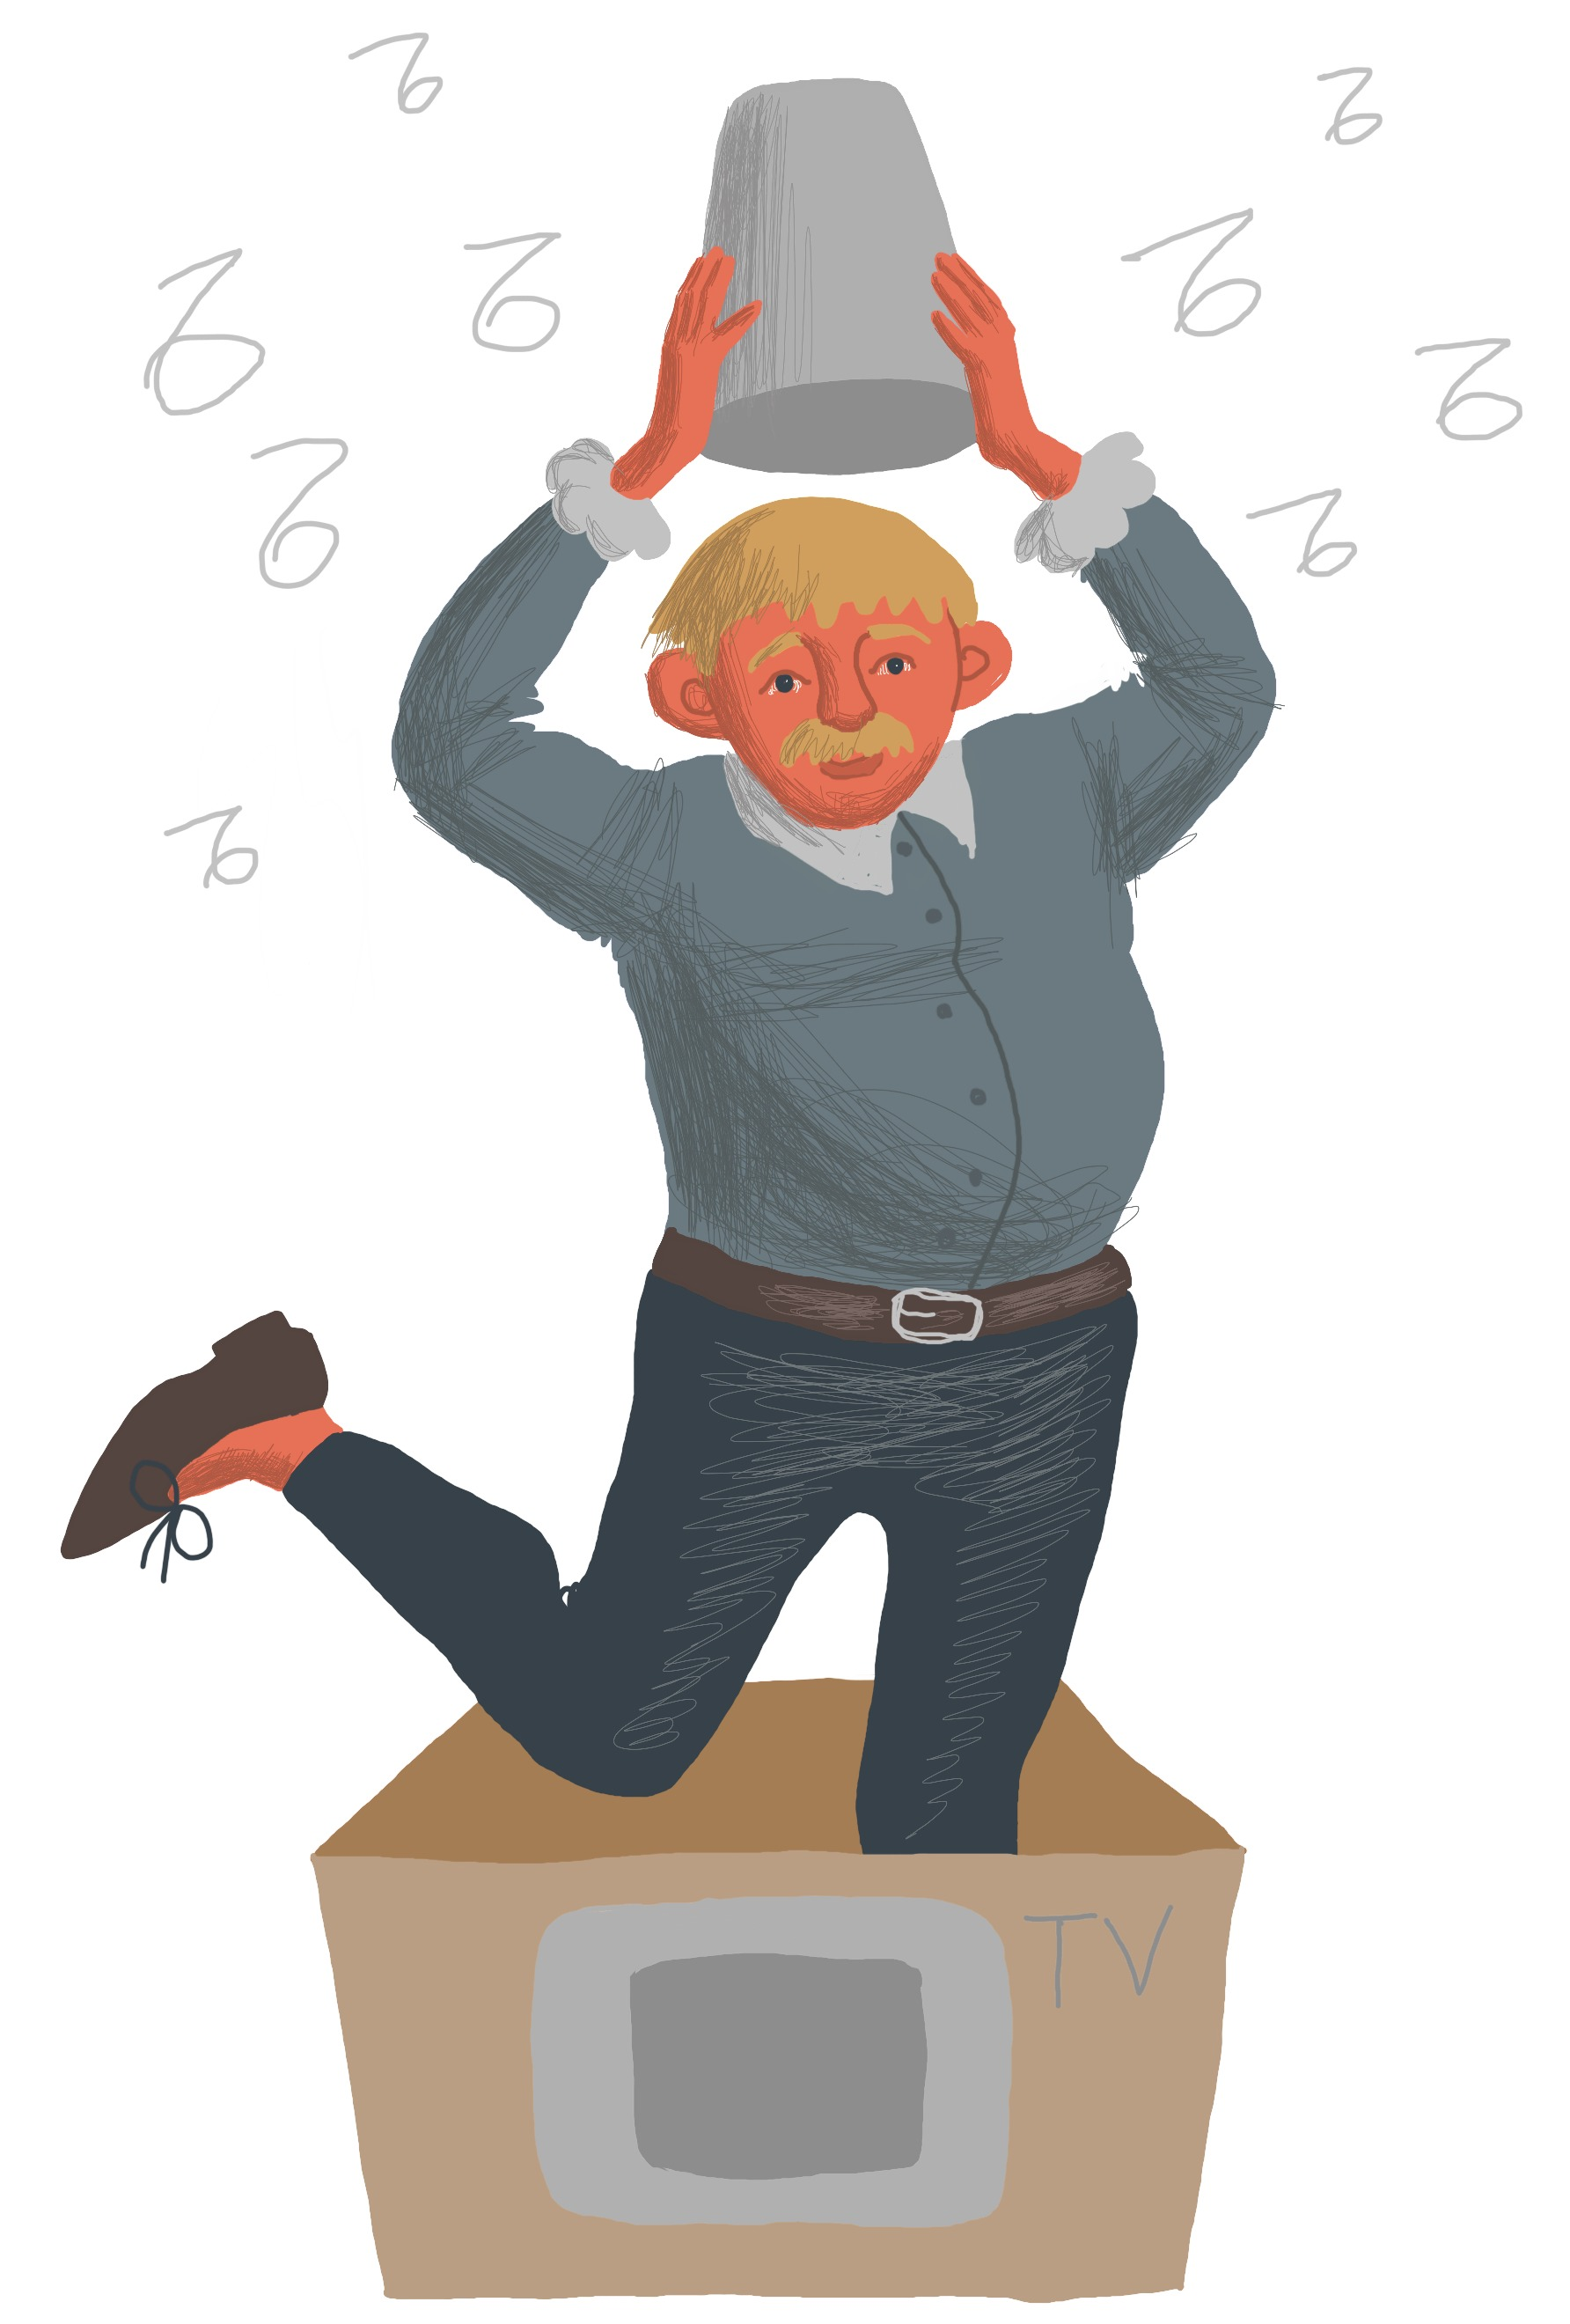
\includegraphics[width=8cm]{figures/color/09c.jpg}
	\vspace{1cm}
	\caption{
             {\itshape  Если сказать мистеру Лэмберту слово <<МАТРАС>>, он кричит <<Караул!>>, 
              снимает перчатки, надевает на голову ведро, встает одной ногой в коробку 
              из-под телевизора и поет два куплета из песни про коня }\medskip\\
             \rightline{Задача 1 <<Летающий цирк>>, 2018 год, 5 класс}}
\end{center} \end{figure}

\begin{figure} \begin{center}
	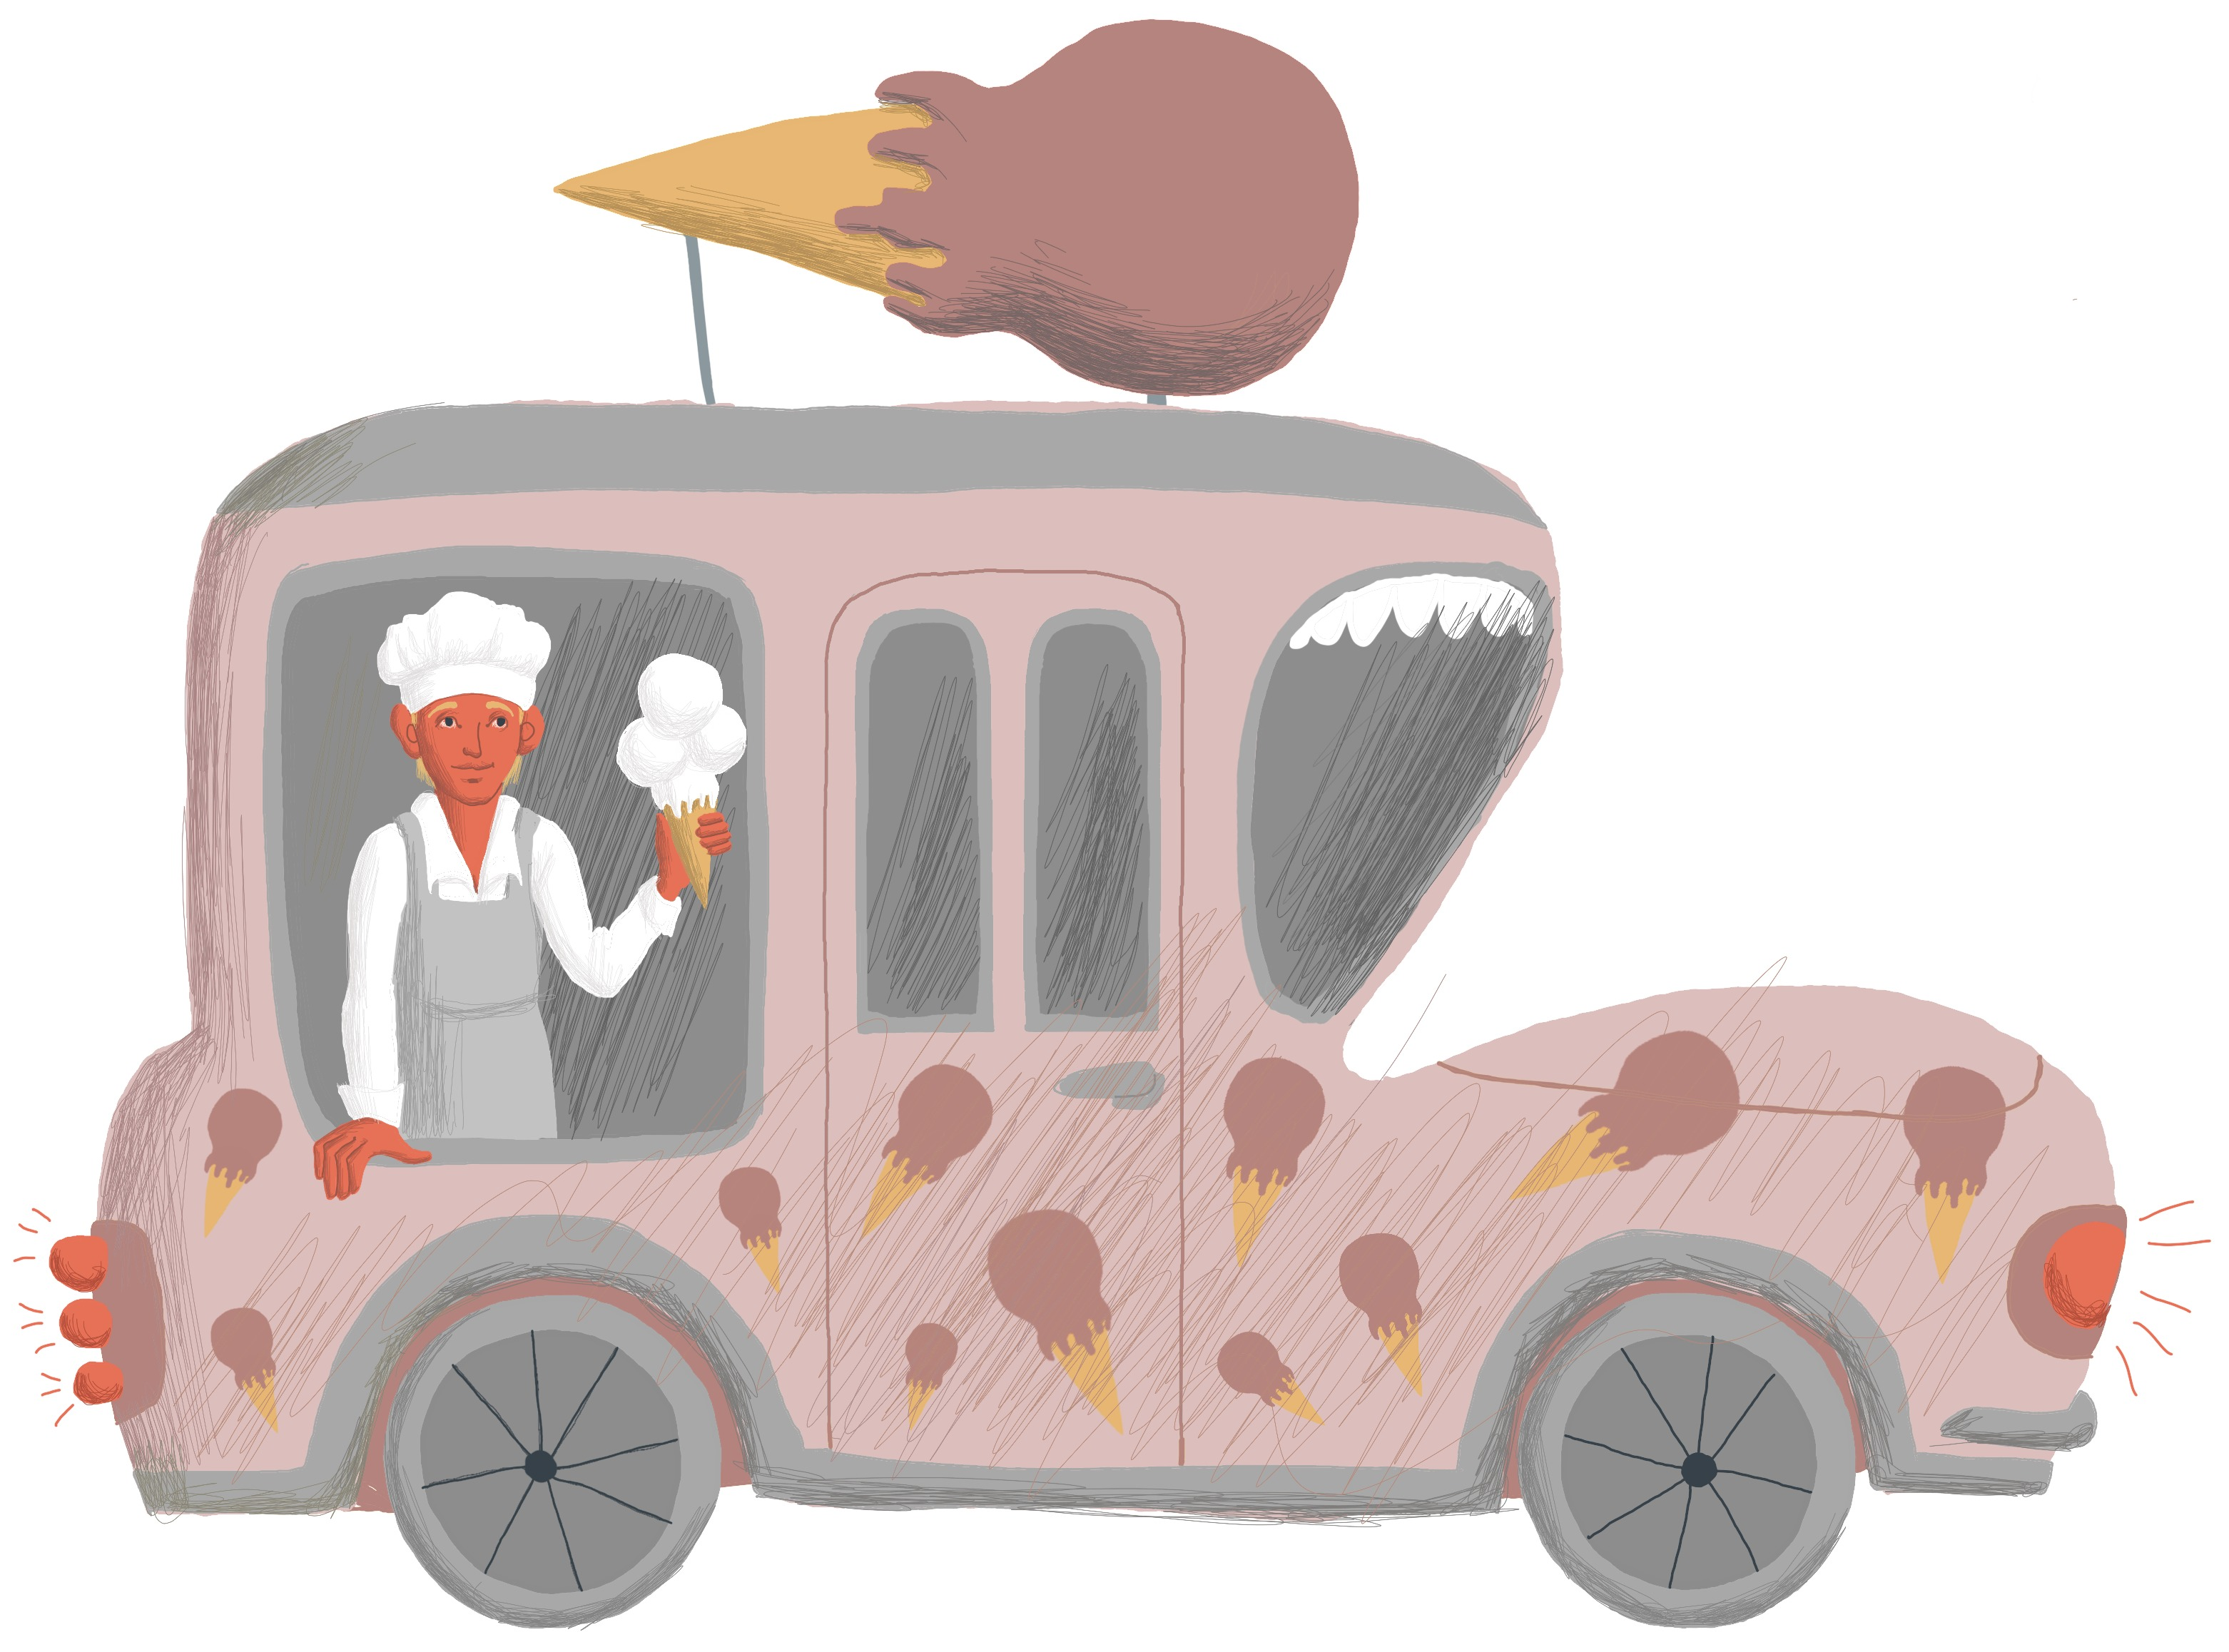
\includegraphics[width=8cm]{figures/color/10c.jpg}
	\vspace{0.5cm}
	\caption{
             {\itshape  Однажды утром мороженщик Саша отправился развозить мороженое 
             на своем новом фургоне }\medskip\\
             \rightline{Задача 8 <<Фургончик>>, 2018 год, 6 класс}}
\end{center} \end{figure}

\begin{figure} \begin{center}
	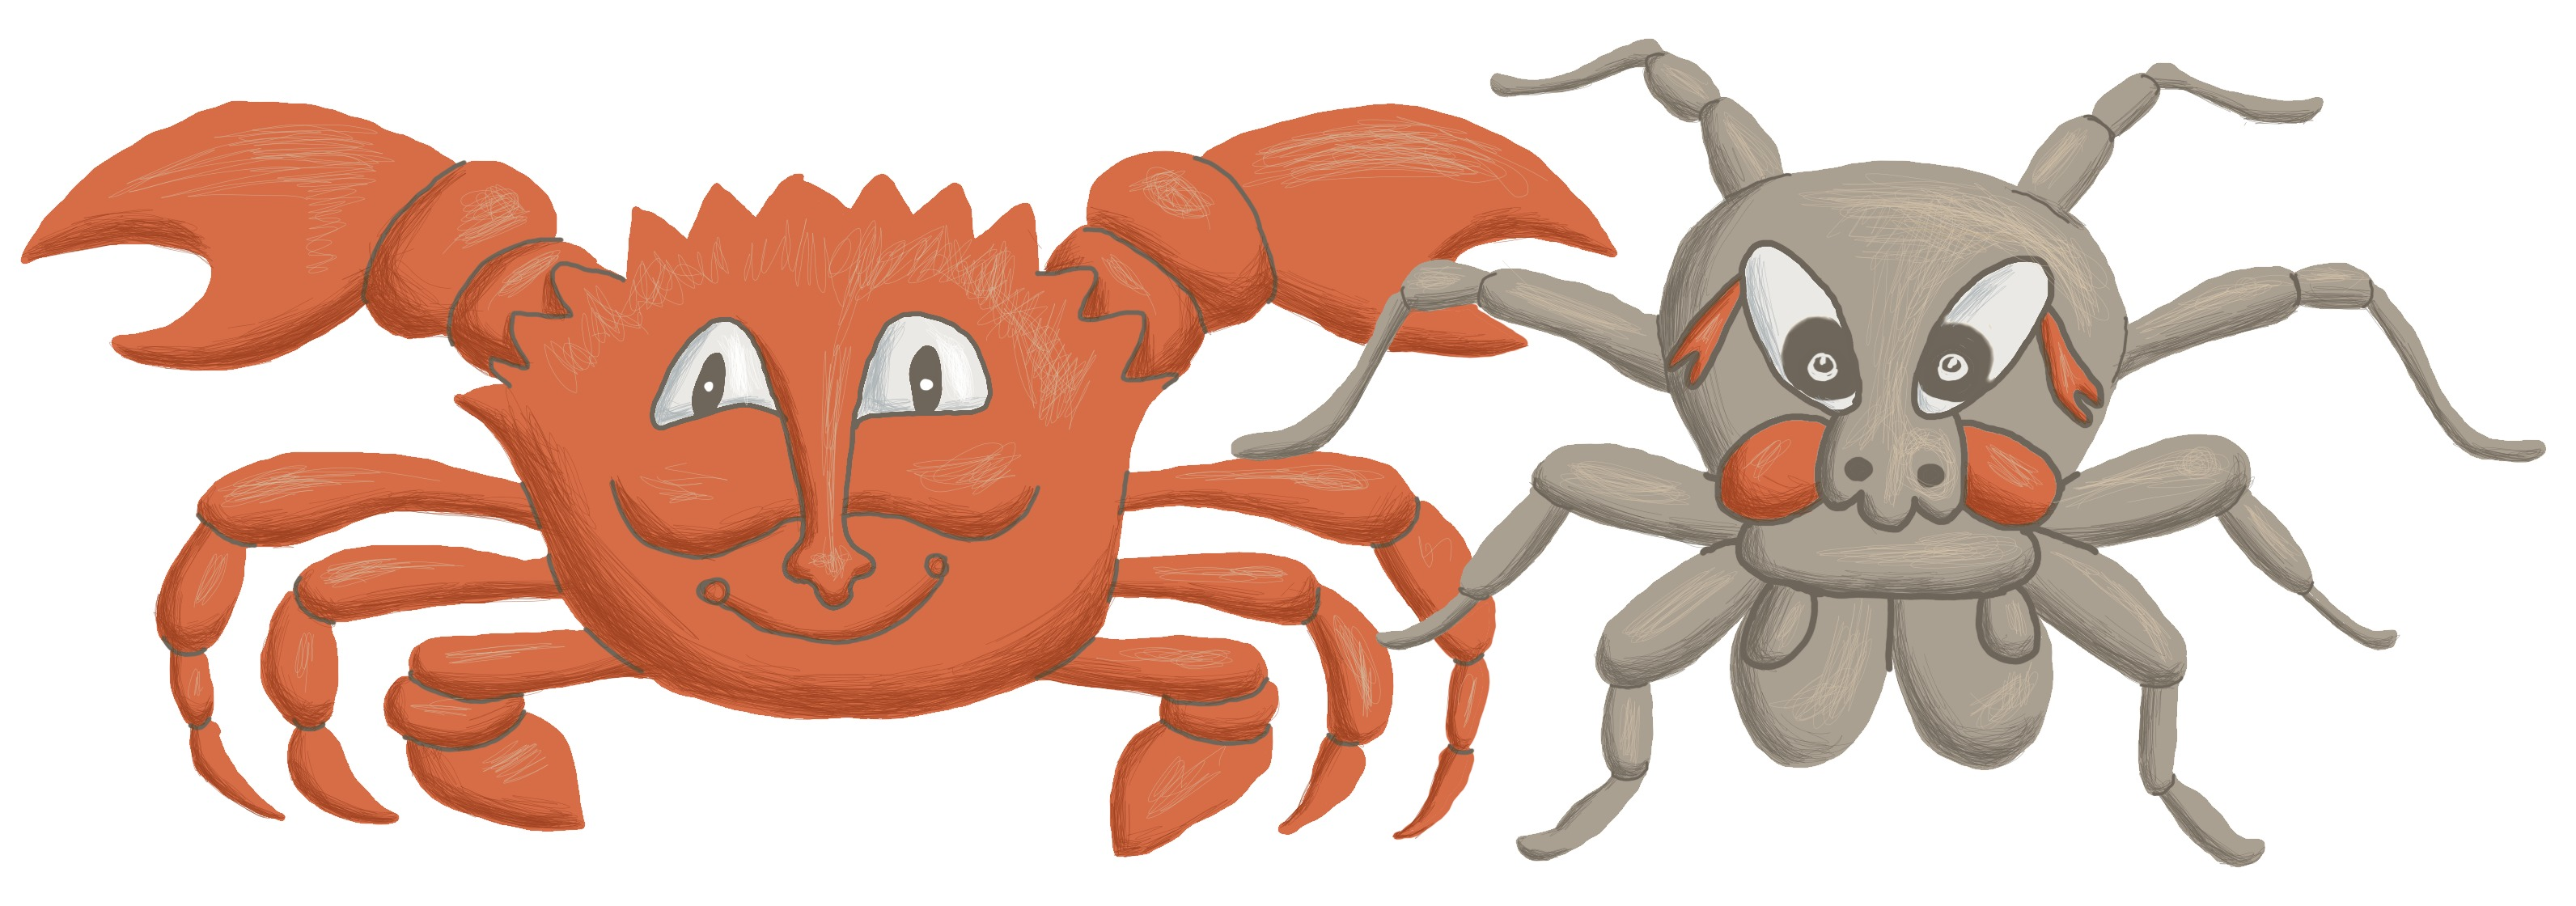
\includegraphics[width=8cm]{figures/color/18c.jpg}
	\vspace{0.5cm}
	\caption{
             {\itshape  Тридцать пять восьминогих существ — 18 крабов и 17 
            пауков — встали в хоровод }\medskip\\
             \rightline{Задача 2 <<Рукопожатия>>, 2018 год, 5 класс}}
\end{center} \end{figure}


\begin{figure} \begin{center}
	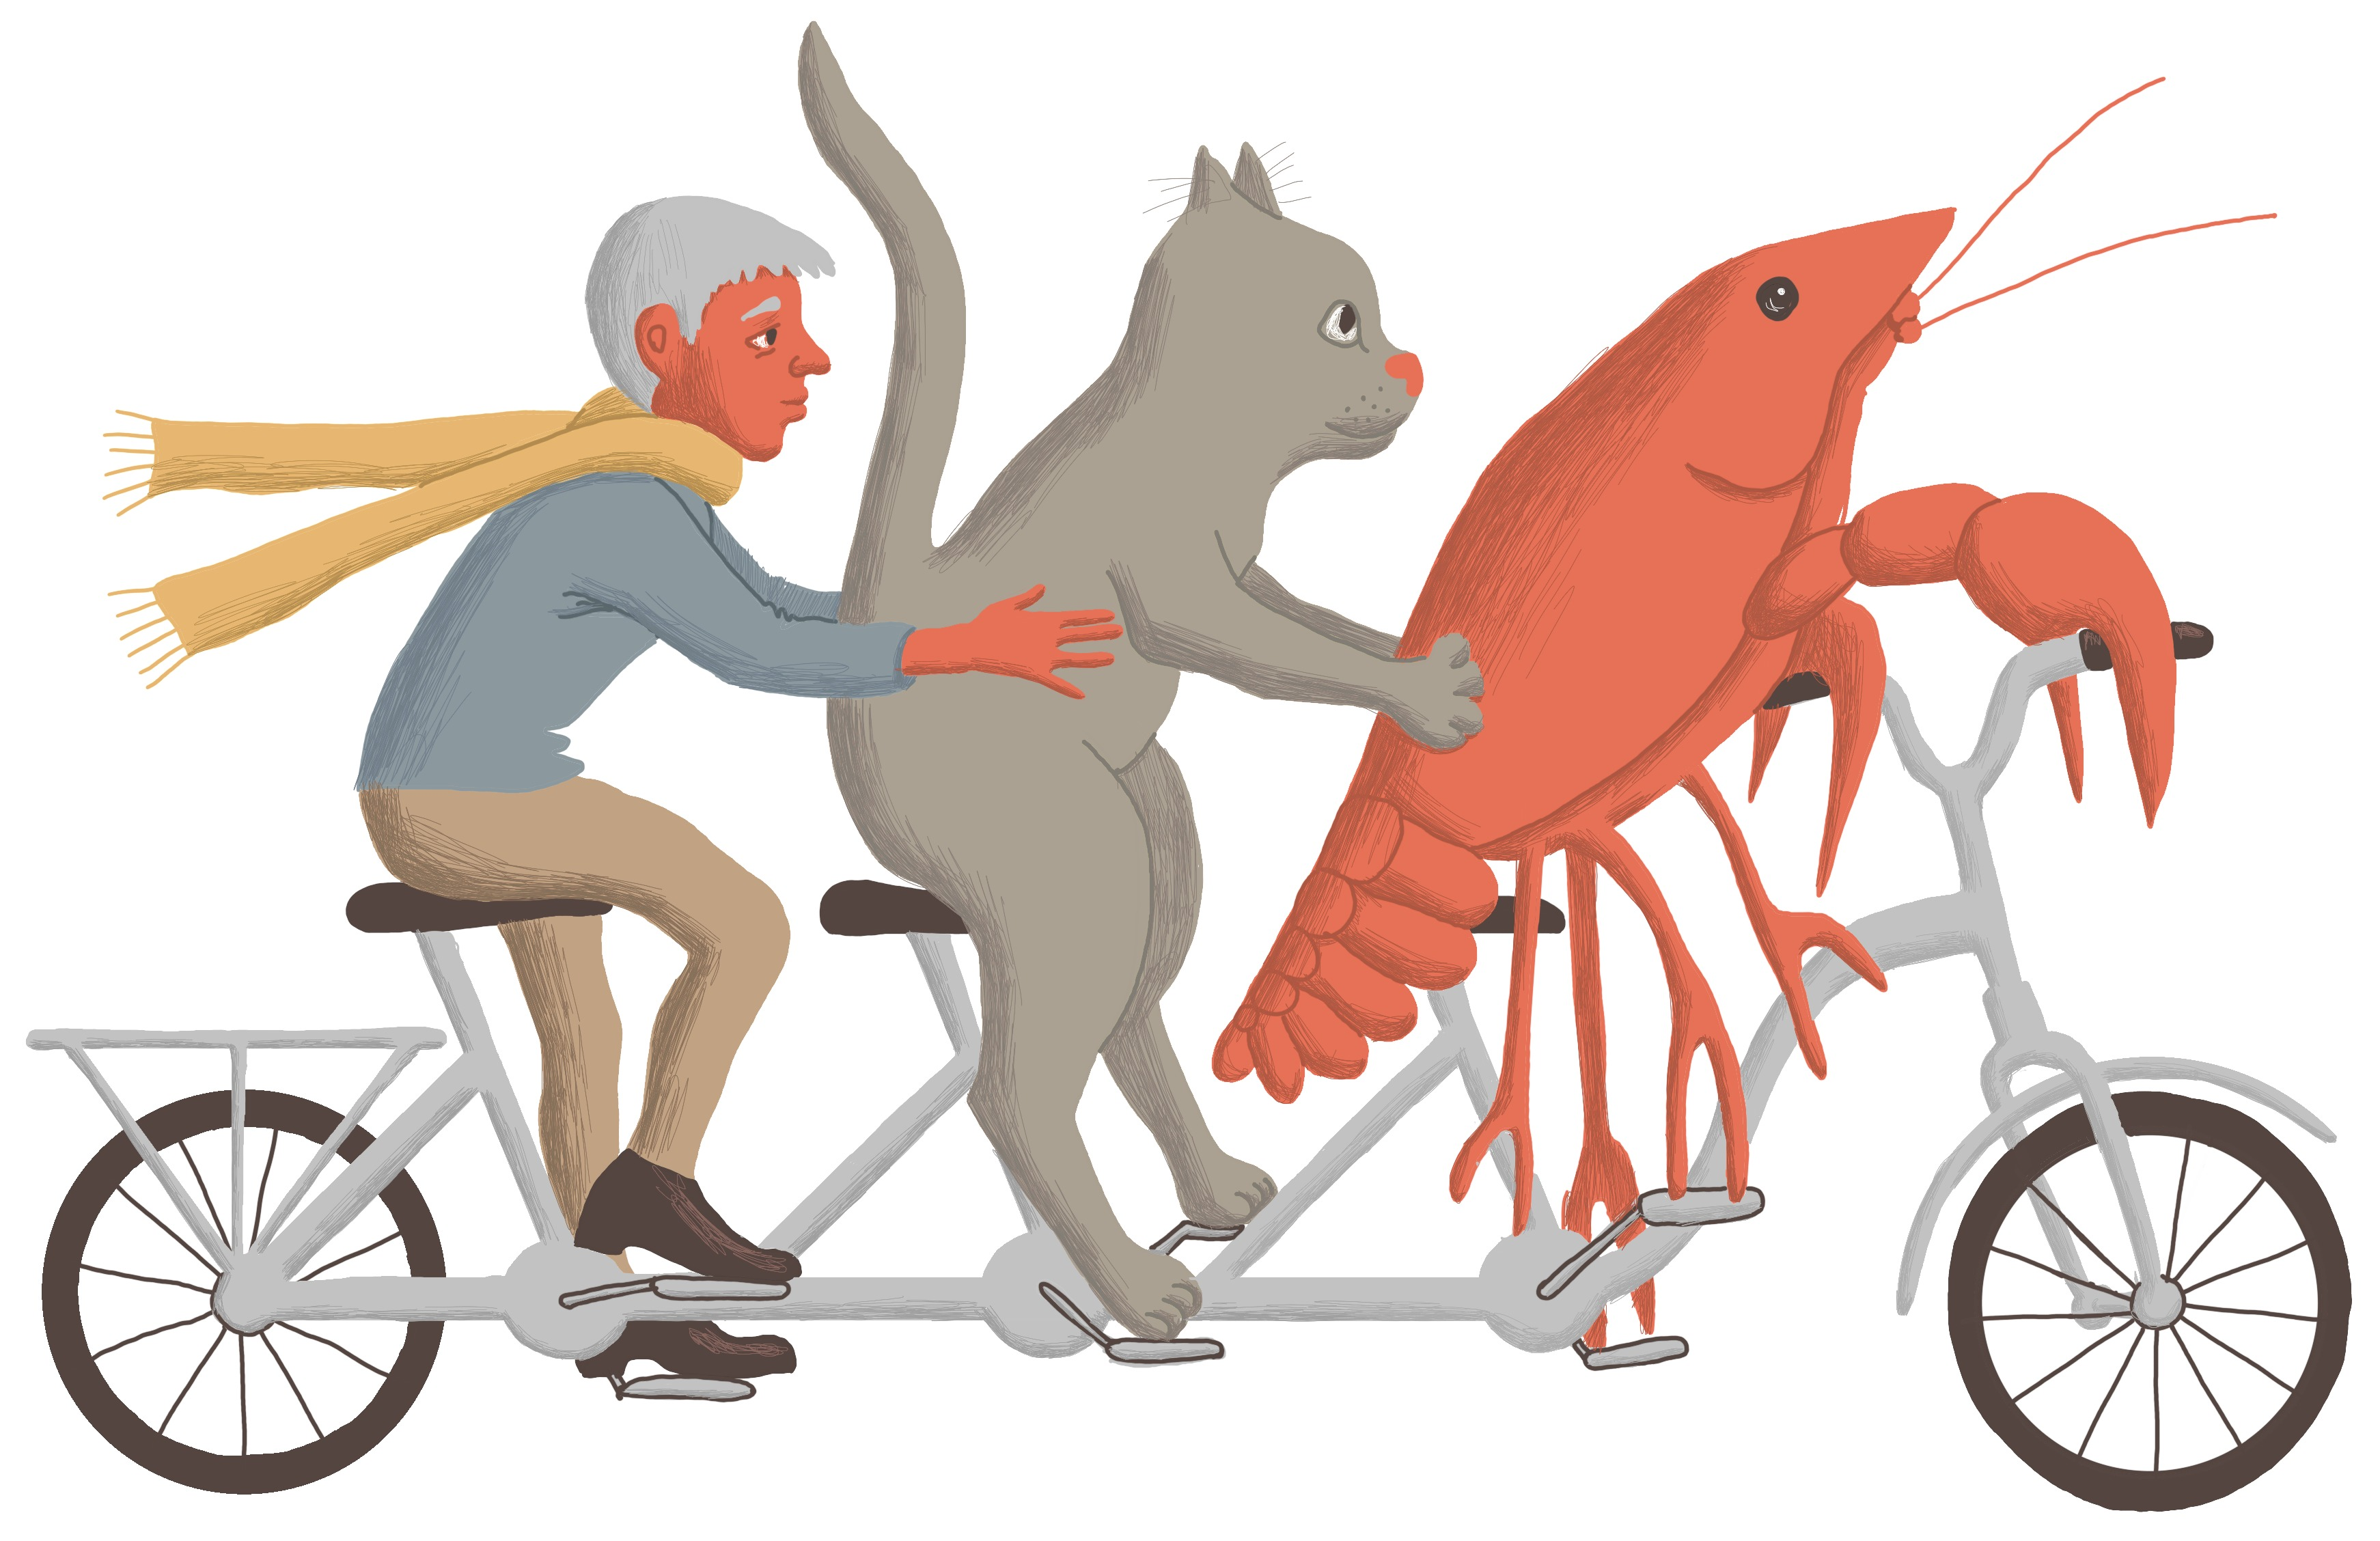
\includegraphics[width=10cm]{figures/color/11c.jpg}
	\vspace{1cm}
	\caption{
             {\itshape  Один коротышка с двумя ногами поехал кататься на велосипеде. 
             Но так как на дворе была зима, $-10$ градусов, он отморозил себе одну ногу ...
             %Другой коротышка через месяц поехал кататься на велосипеде. Но на дворе по-прежнему 
             %была зима, уже $-20$ градусов, и он отморозил себе все имеющиеся ноги (их также было две).
             Сколько ног отморозит себе на 10- и на 20-градусном морозе туристическая группа из 
             40 коротышек? А их маленький серый кот, у которого ног изначально четыре? 
             А речной рак, у которого восемь ног? }\medskip\\
             \rightline{Задача 2 <<Напрасно называют север крайним>>,}\\
             \rightline{2018 год, 4 класс}}
\end{center} \end{figure}

\begin{figure} \begin{center}
	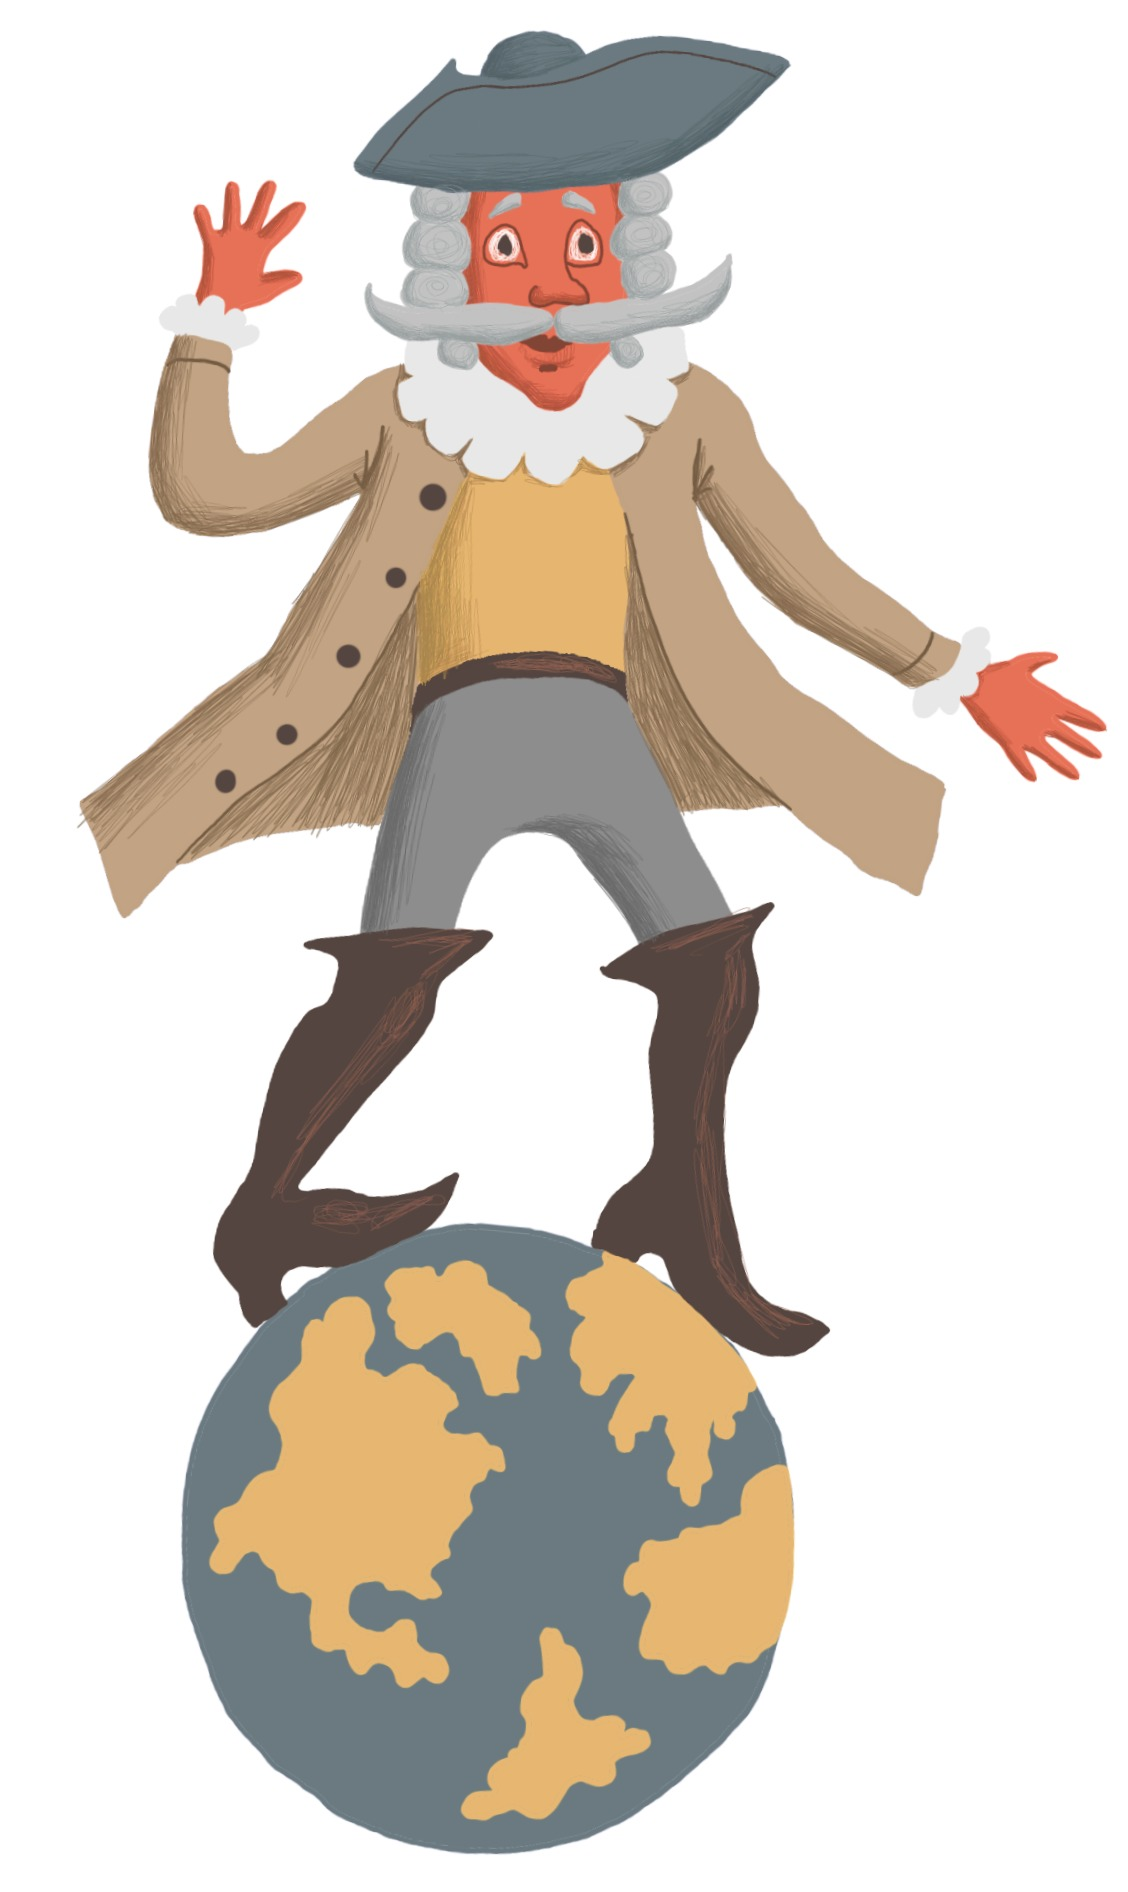
\includegraphics[width=8cm]{figures/color/12c.jpg}
	\vspace{1cm}
	\caption{
             {\itshape  Барон Мюнхгаузен говорит, что обошел вокруг света (то есть побывал на 
              всех возможных долготах Земного шара) за 40 минут. При этом известно, что он не лжет. 
              Как такое могло произойти? }\medskip\\
             \rightline{Задача 2 <<Напрасно называют север крайним>>}\\
             \rightline{2018 год, 4 класс}}
\end{center} \end{figure}


\begin{figure} \begin{center}
	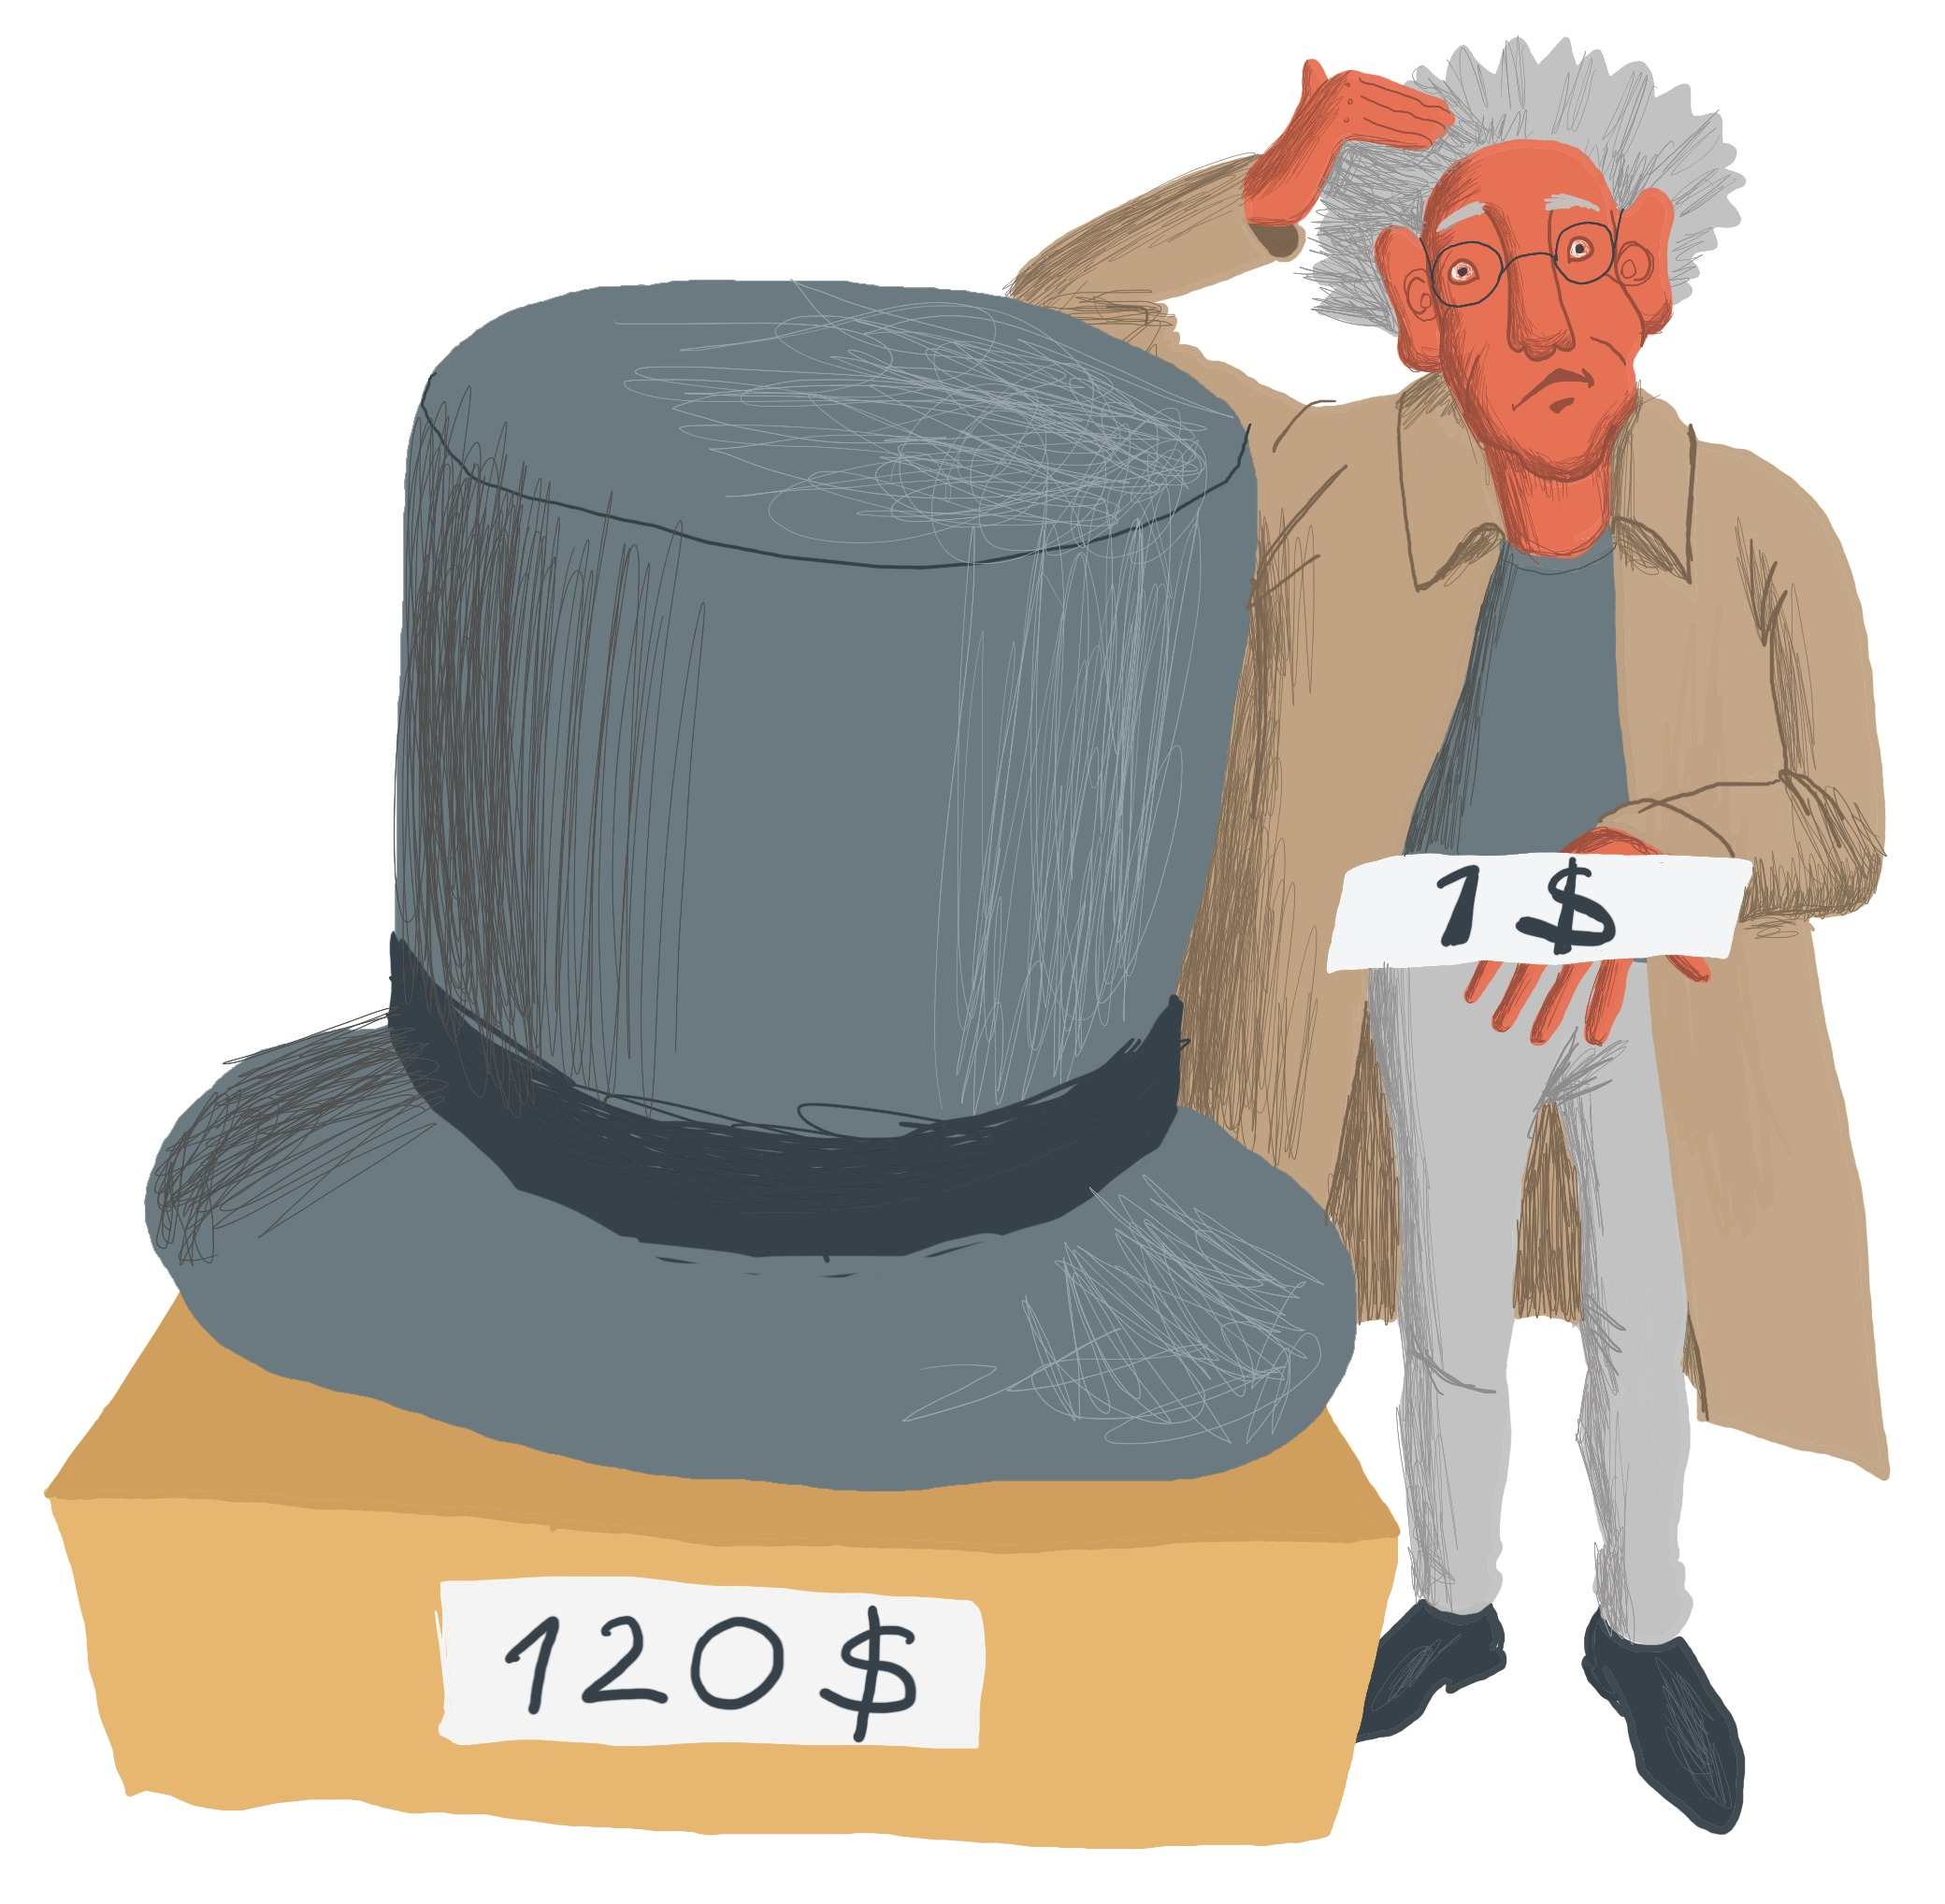
\includegraphics[width=10cm]{figures/color/13c.jpg}
	\vspace{1cm}
	\caption{
             {\itshape  Сможет ли джентльмен когда-нибудь купить себе желанную шляпу? }\medskip\\
             {Задача 1 <<Летающий цирк>>, 2018 год, 5 класс}}
\end{center} \end{figure}

\begin{figure} \begin{center}
	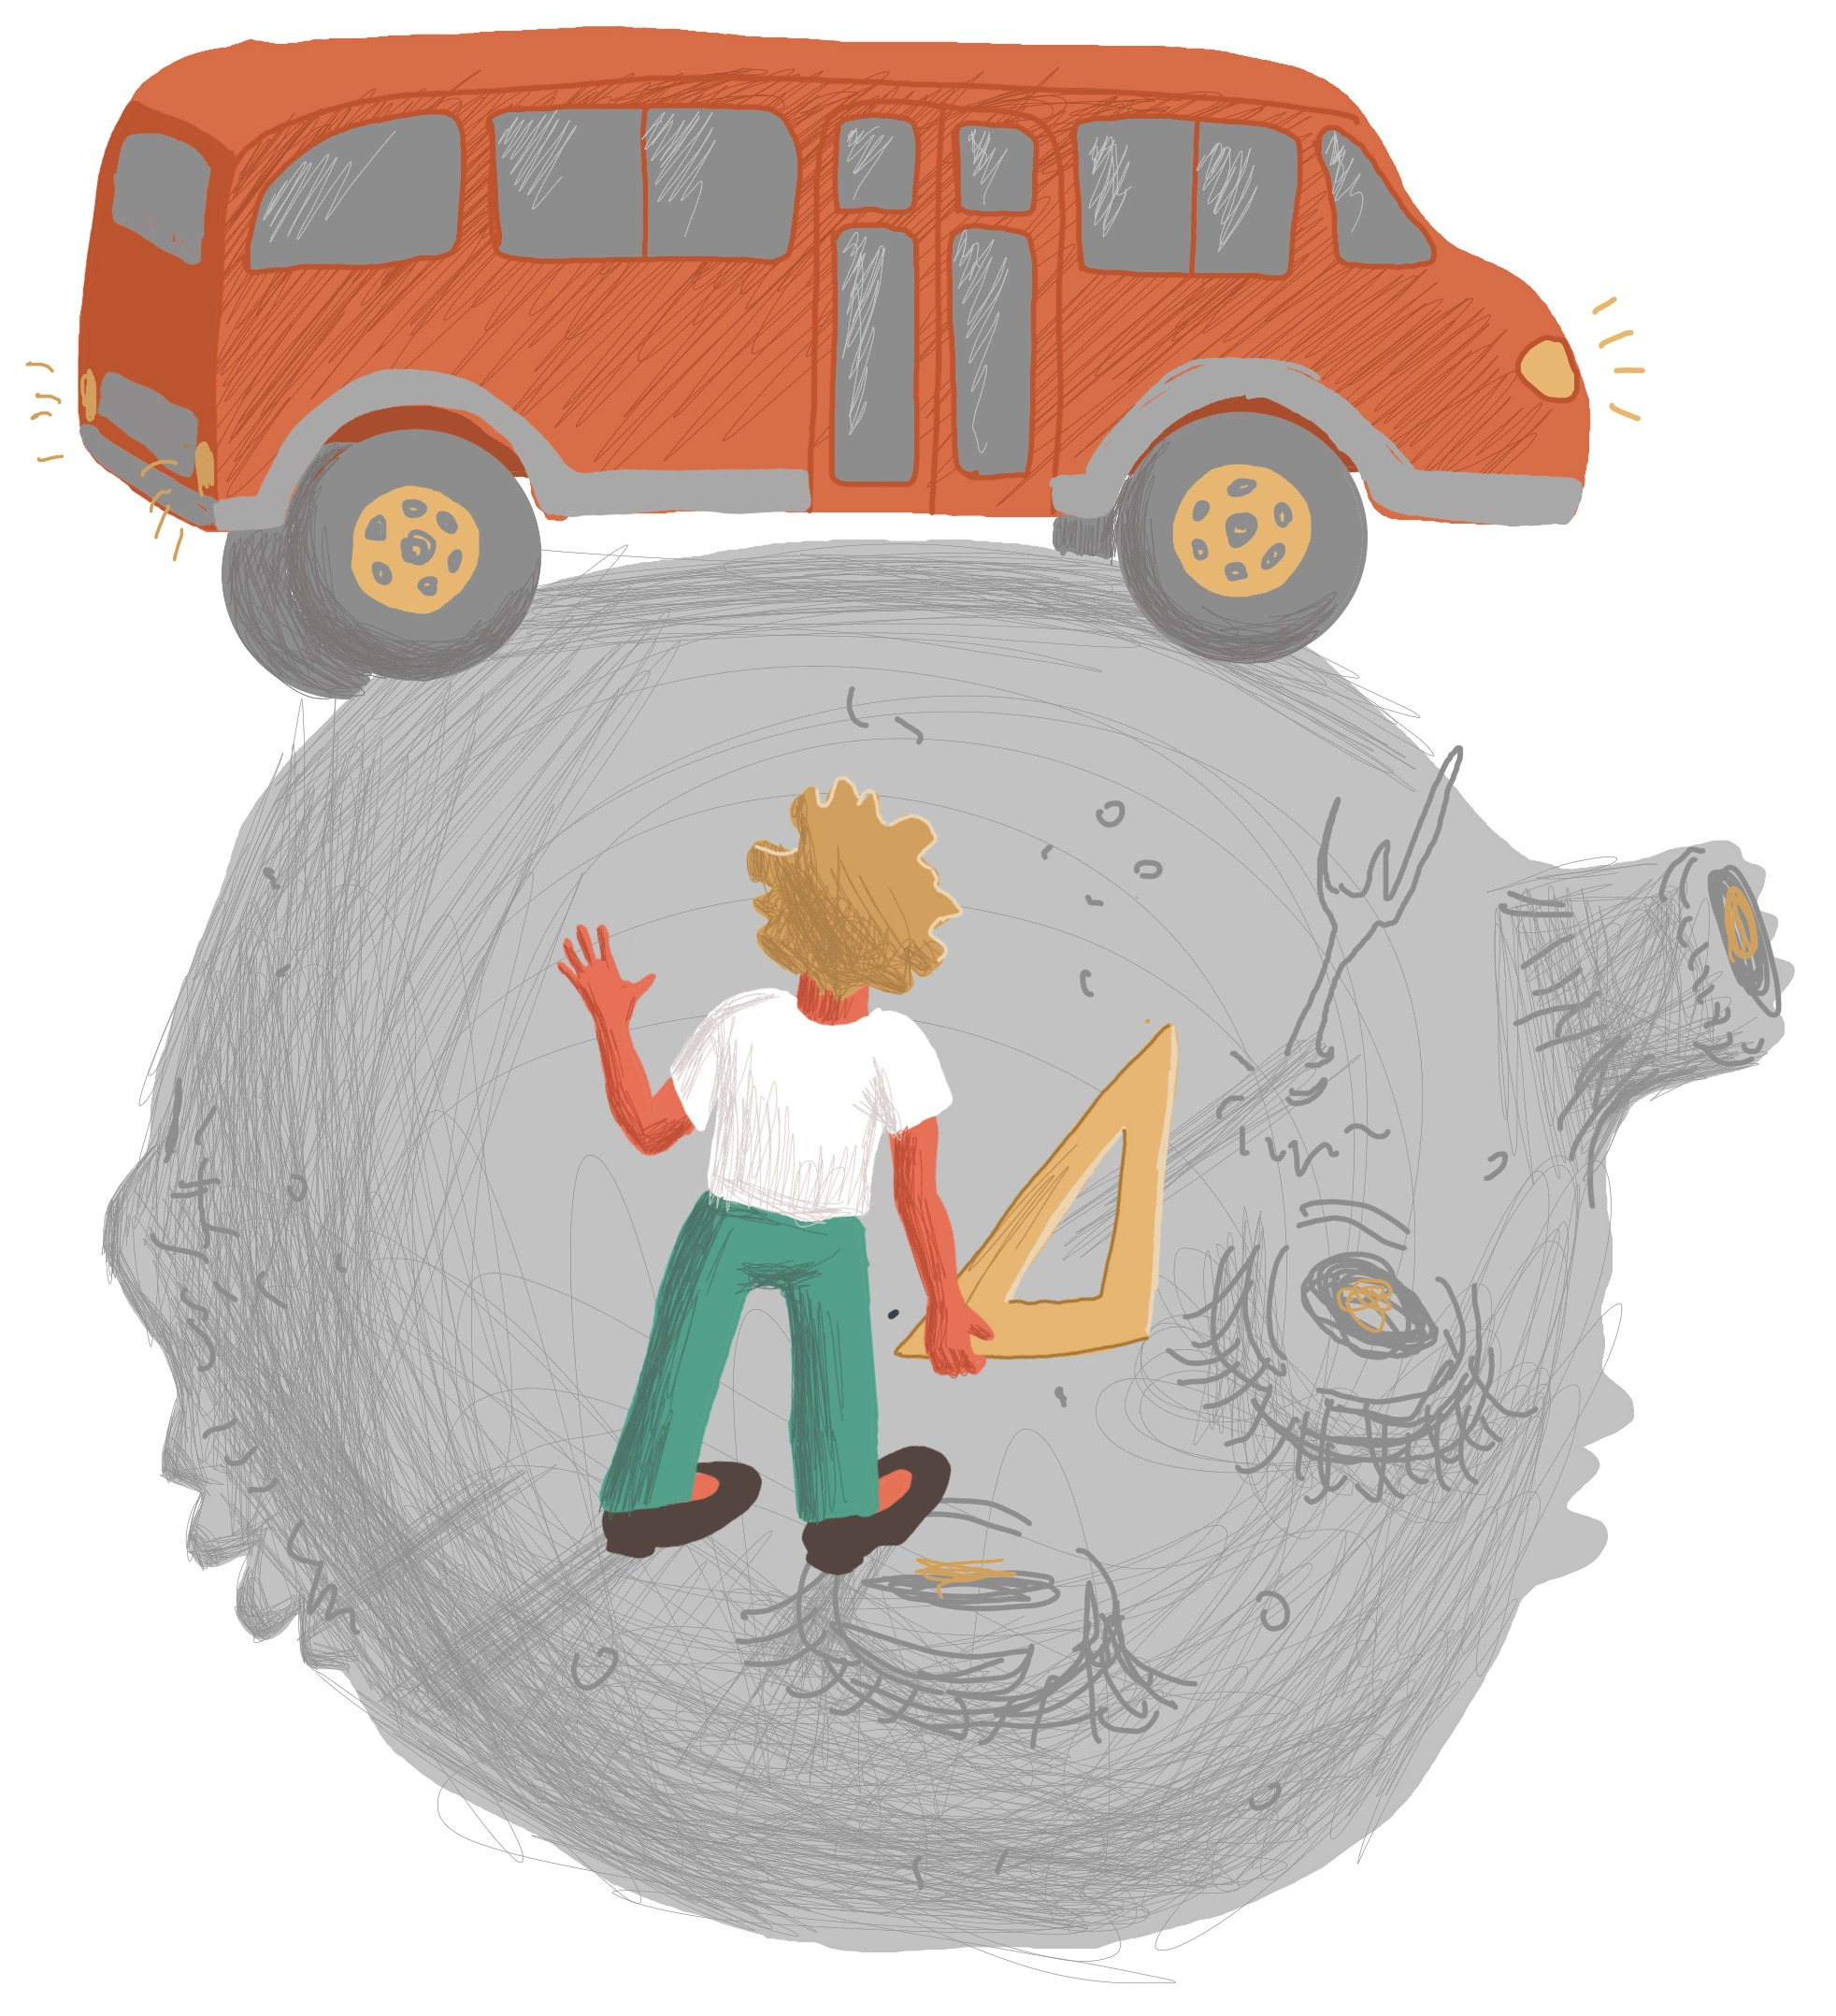
\includegraphics[width=10cm]{figures/color/14c.jpg}
	\vspace{1cm}
	\caption{
             {\itshape  Автобус с диаметром колес 1 метр и колесной базой $10.5$ метров 
             (так называют расстояние между передней осью и задней) стоит на планете Маленького 
             принца, диаметр которой 20 метров }\medskip\\
             \rightline{Задача 1 <<Клиренсы>>, 2018 год, 6 класс}}
\end{center} \end{figure}

\begin{figure} \begin{center}
	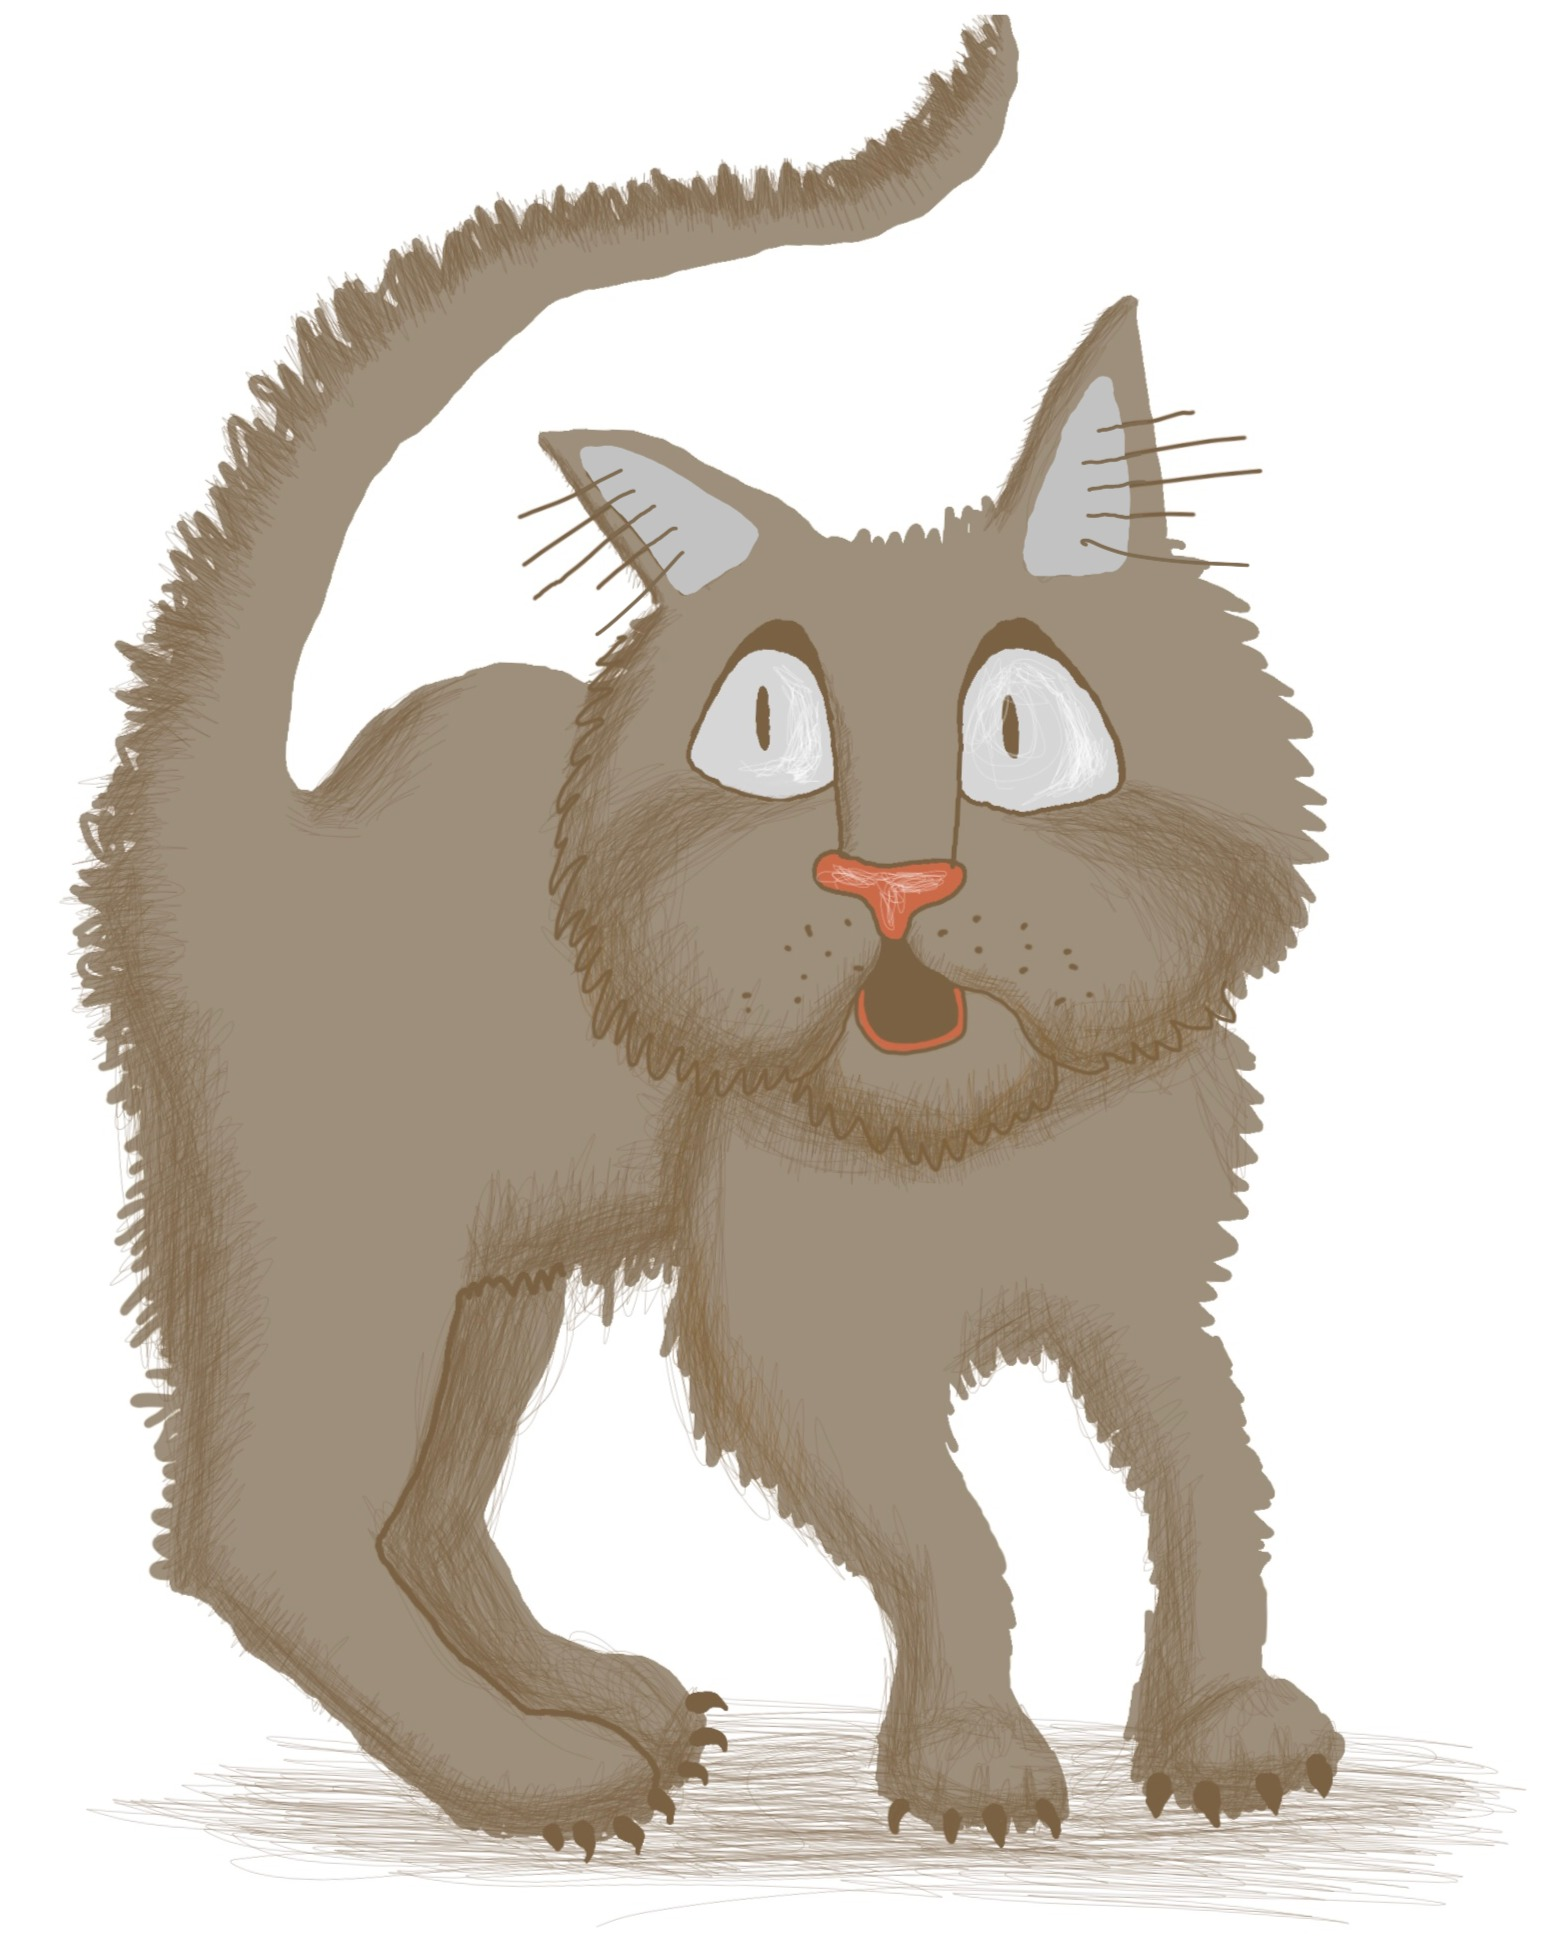
\includegraphics[width=10cm]{figures/color/16c.jpg}
	\vspace{1cm}
	\caption{
             {\itshape Тревор: «Этот сконфуженный кот стоит 9600 рублей»}\medskip\\
             \rightline{Задача 1 <<Летающий цирк>>, 2018 год, 5 класс}}
\end{center} \end{figure}

\begin{figure} \begin{center}
	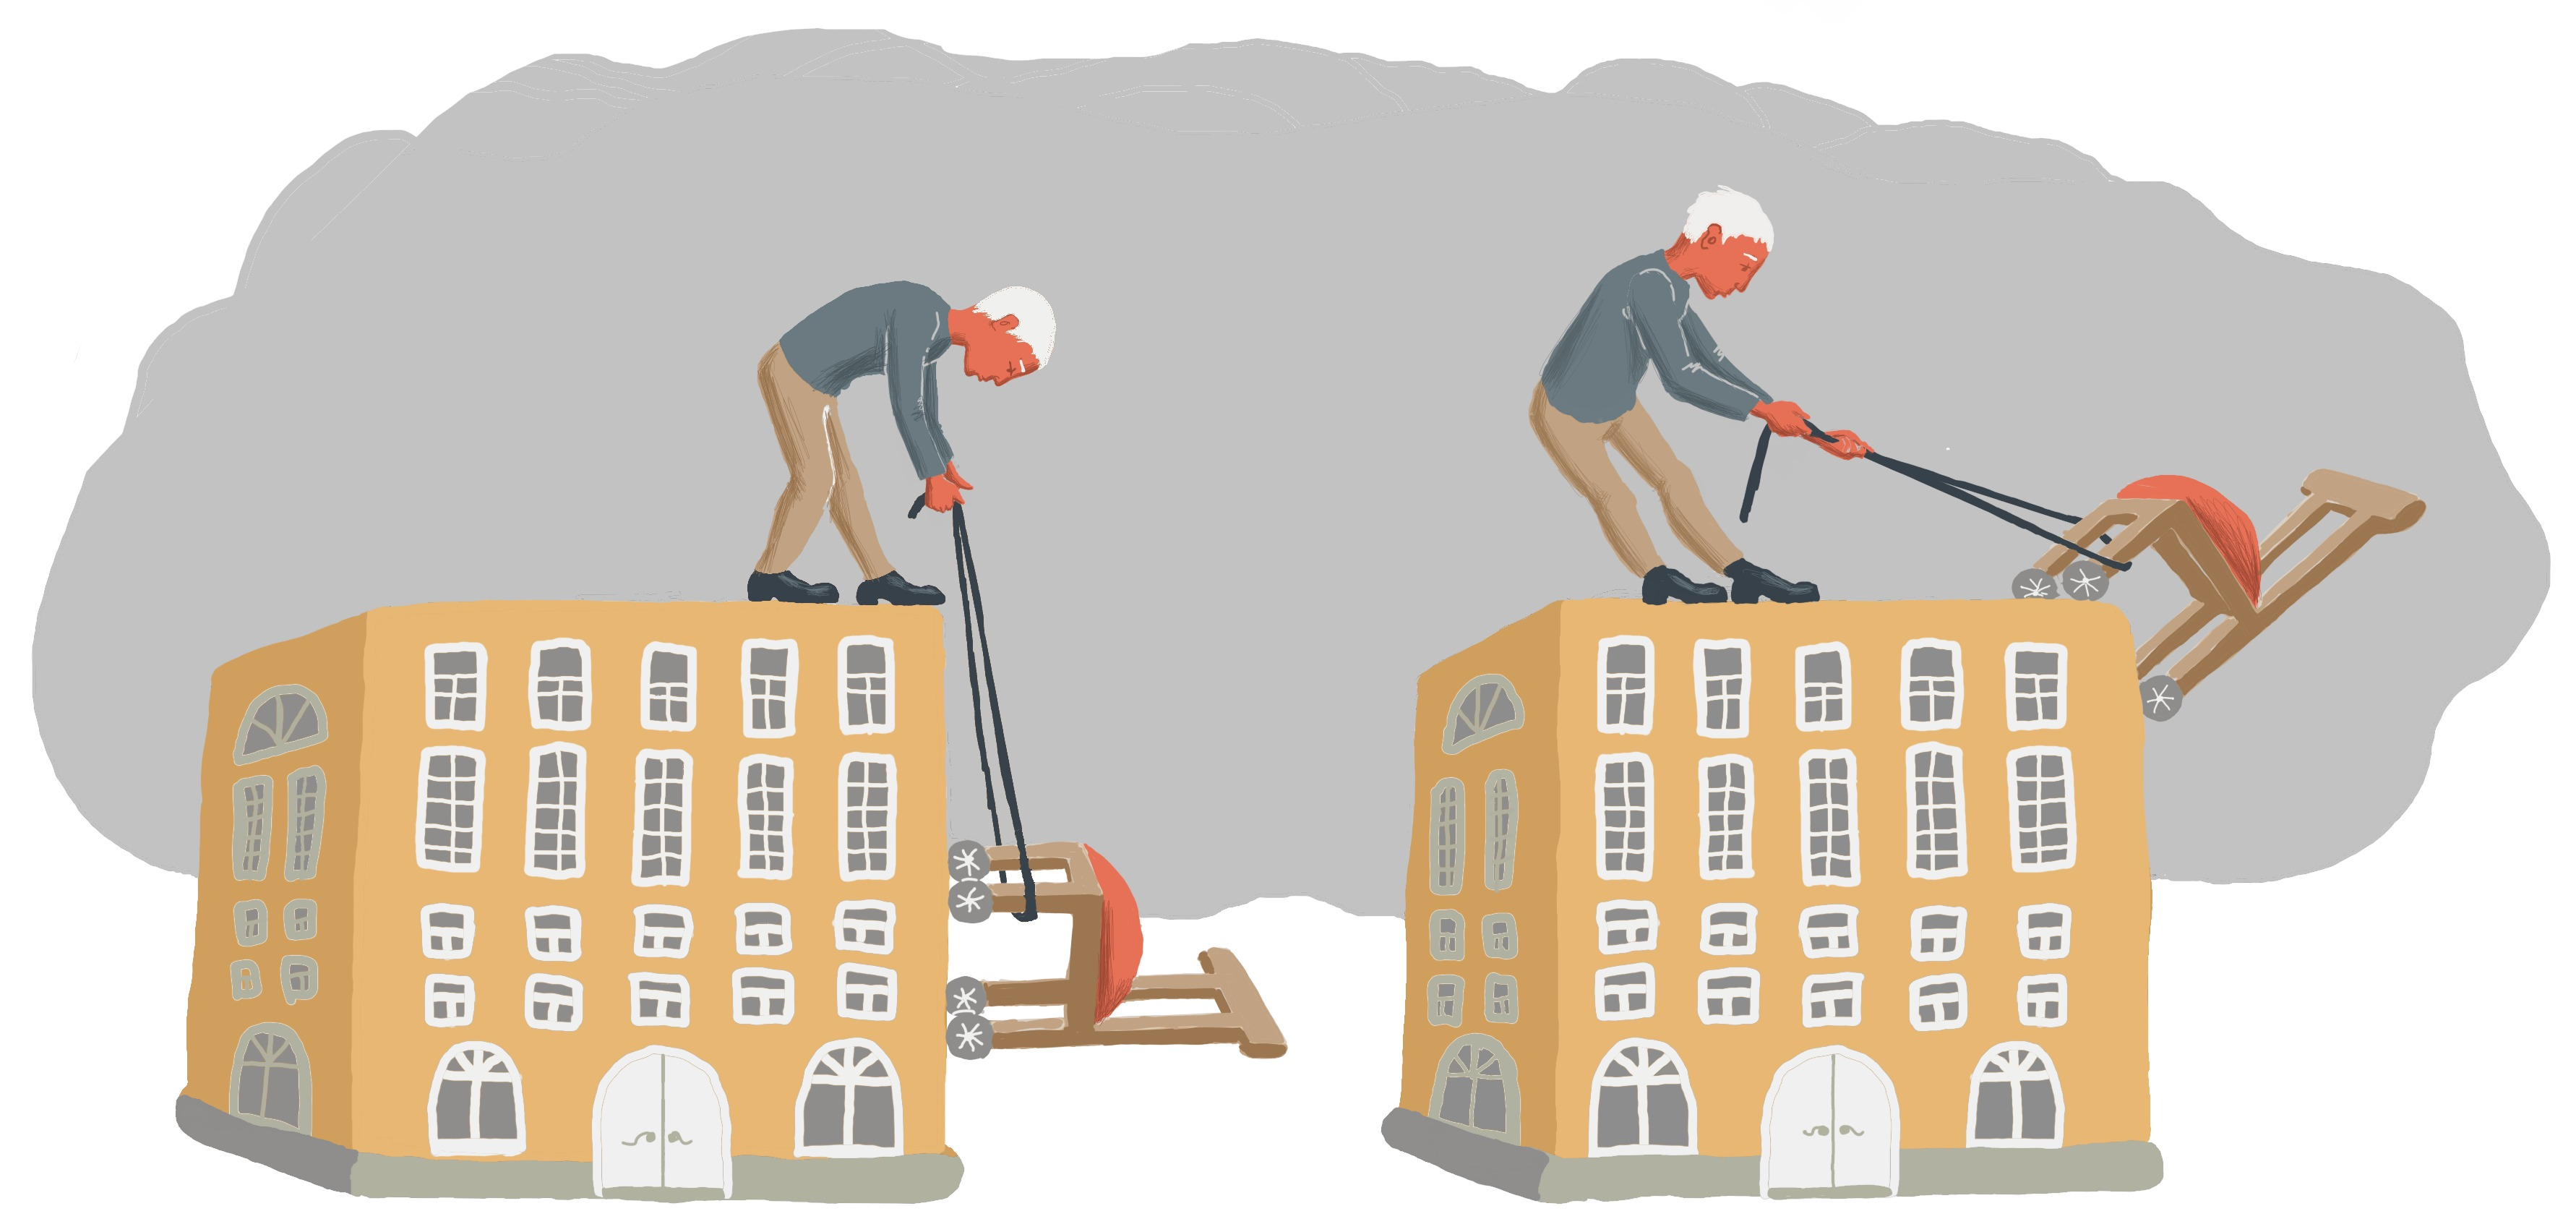
\includegraphics[width=8cm]{figures/color/17c.jpg}
	\vspace{0.5cm}
	\caption{
             {\itshape  Расстояние между соседними ножками стула — 50 см. 
             К ножкам стула прикрепили колесики и стали втаскивать его за 
             веревку по стене многоэтажного дома, который имеет форму куба, 
             так, что стул едет по стене колесиками }\medskip\\
             \rightline{Задача 1 <<Клиренсы>>, 2018 год, 6 класс}}
\end{center} \end{figure}

\begin{figure} \begin{center}
	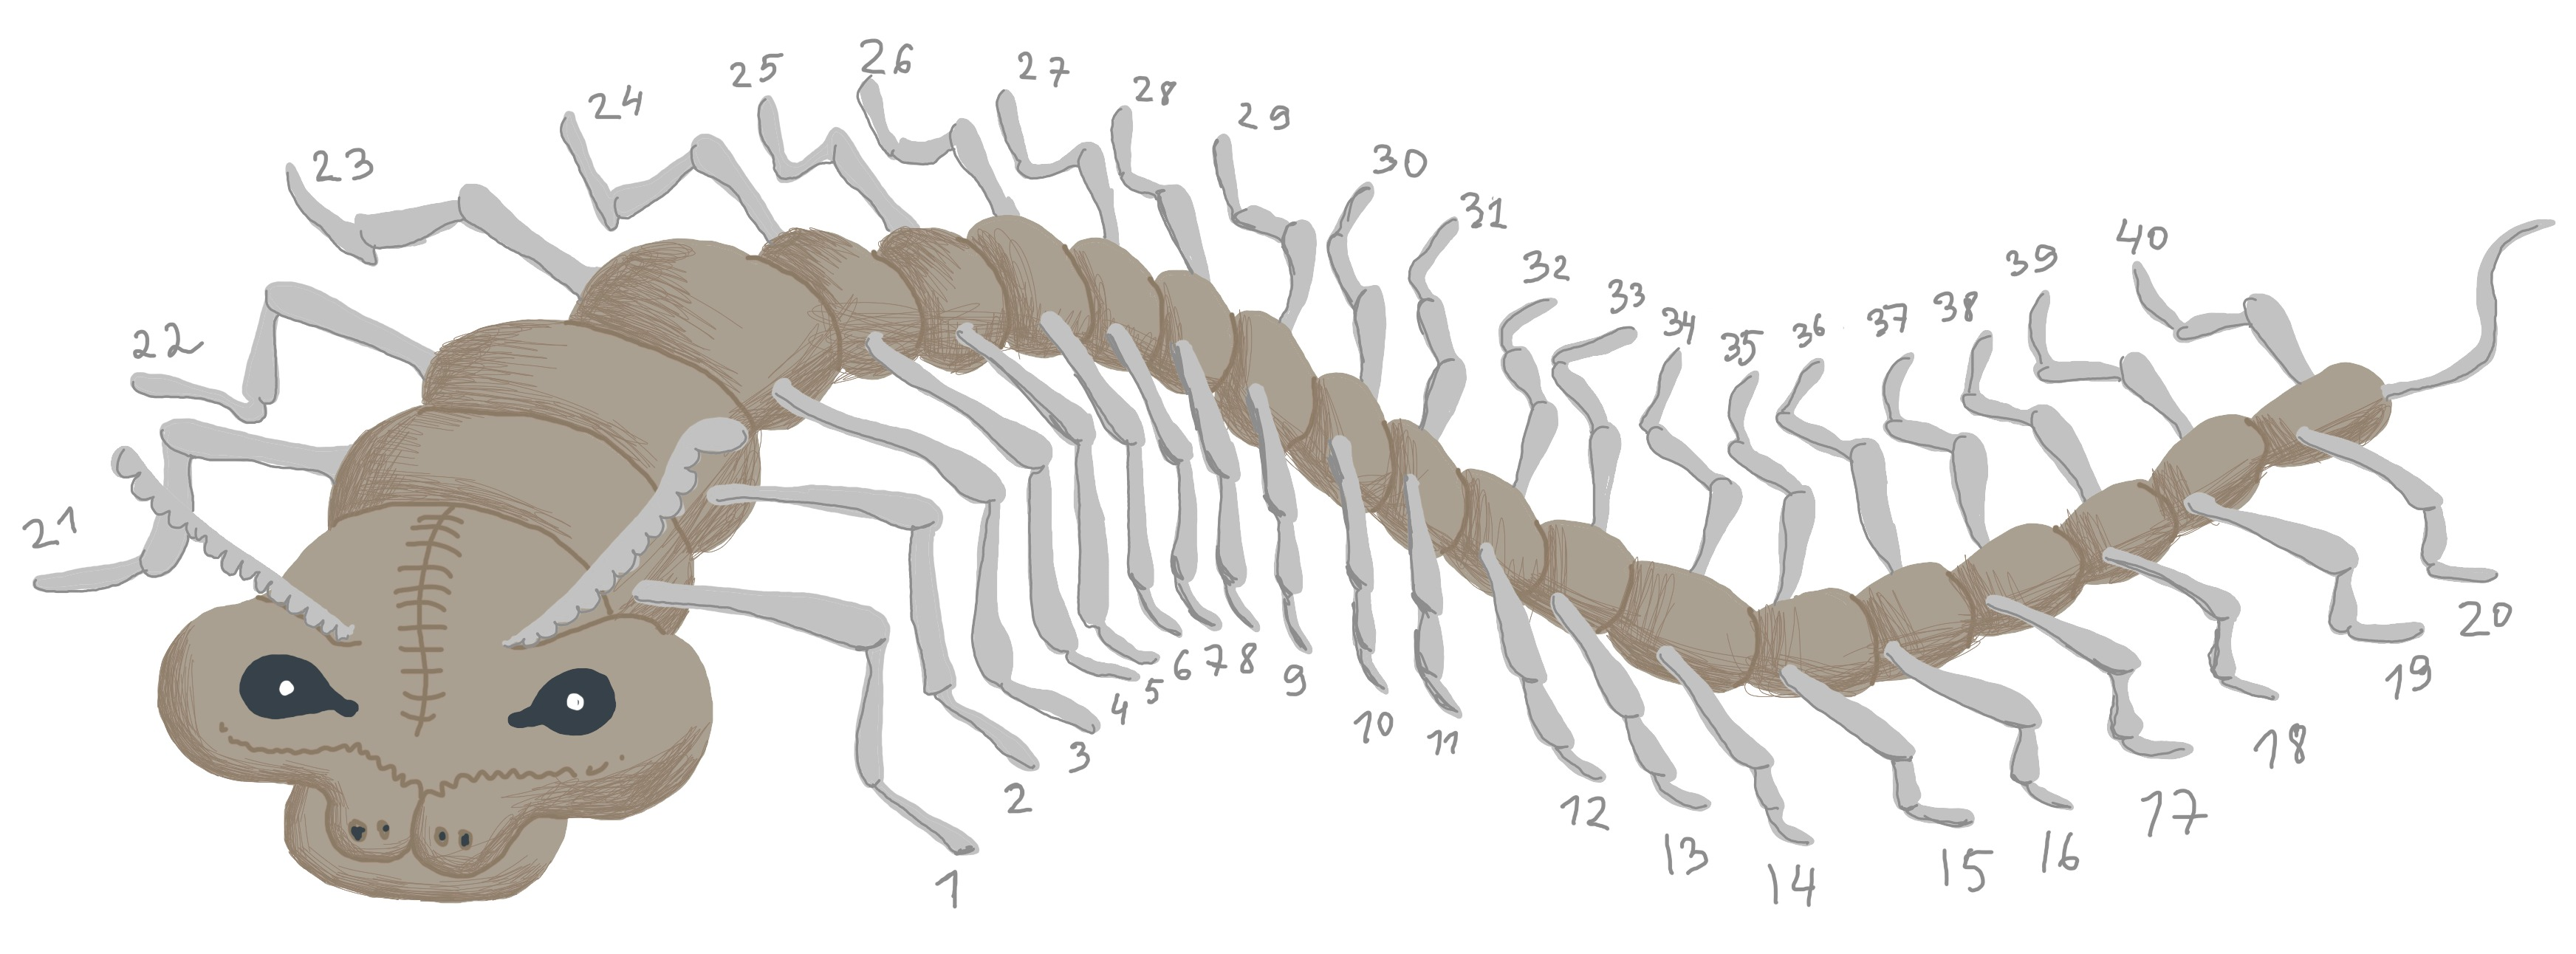
\includegraphics[width=8cm]{figures/color/08c.jpg}
	\vspace{0.5cm}
	\caption{
             {\itshape  В сашином фургоне родилась сороконожка (ее ноги пронумерованы от 1 до 40). 
              Она хочет сделать первый шаг — и переставляет первую ногу. 
              %Вторым шагом она переставляет все ноги, номера которых делятся на~2. 
              %Третьим — все ноги, номера которых делятся на 3 и которые не были переставлены ранее. 
              %Сколько ног ей теперь осталось переставить, чтобы окончательно сдвинуться с места? 
             }\medskip\\
             \rightline{Задача 8 <<Фургончик>>, 2018 год, 6 класс}}
\end{center} \end{figure}

\begin{figure} \begin{center}
	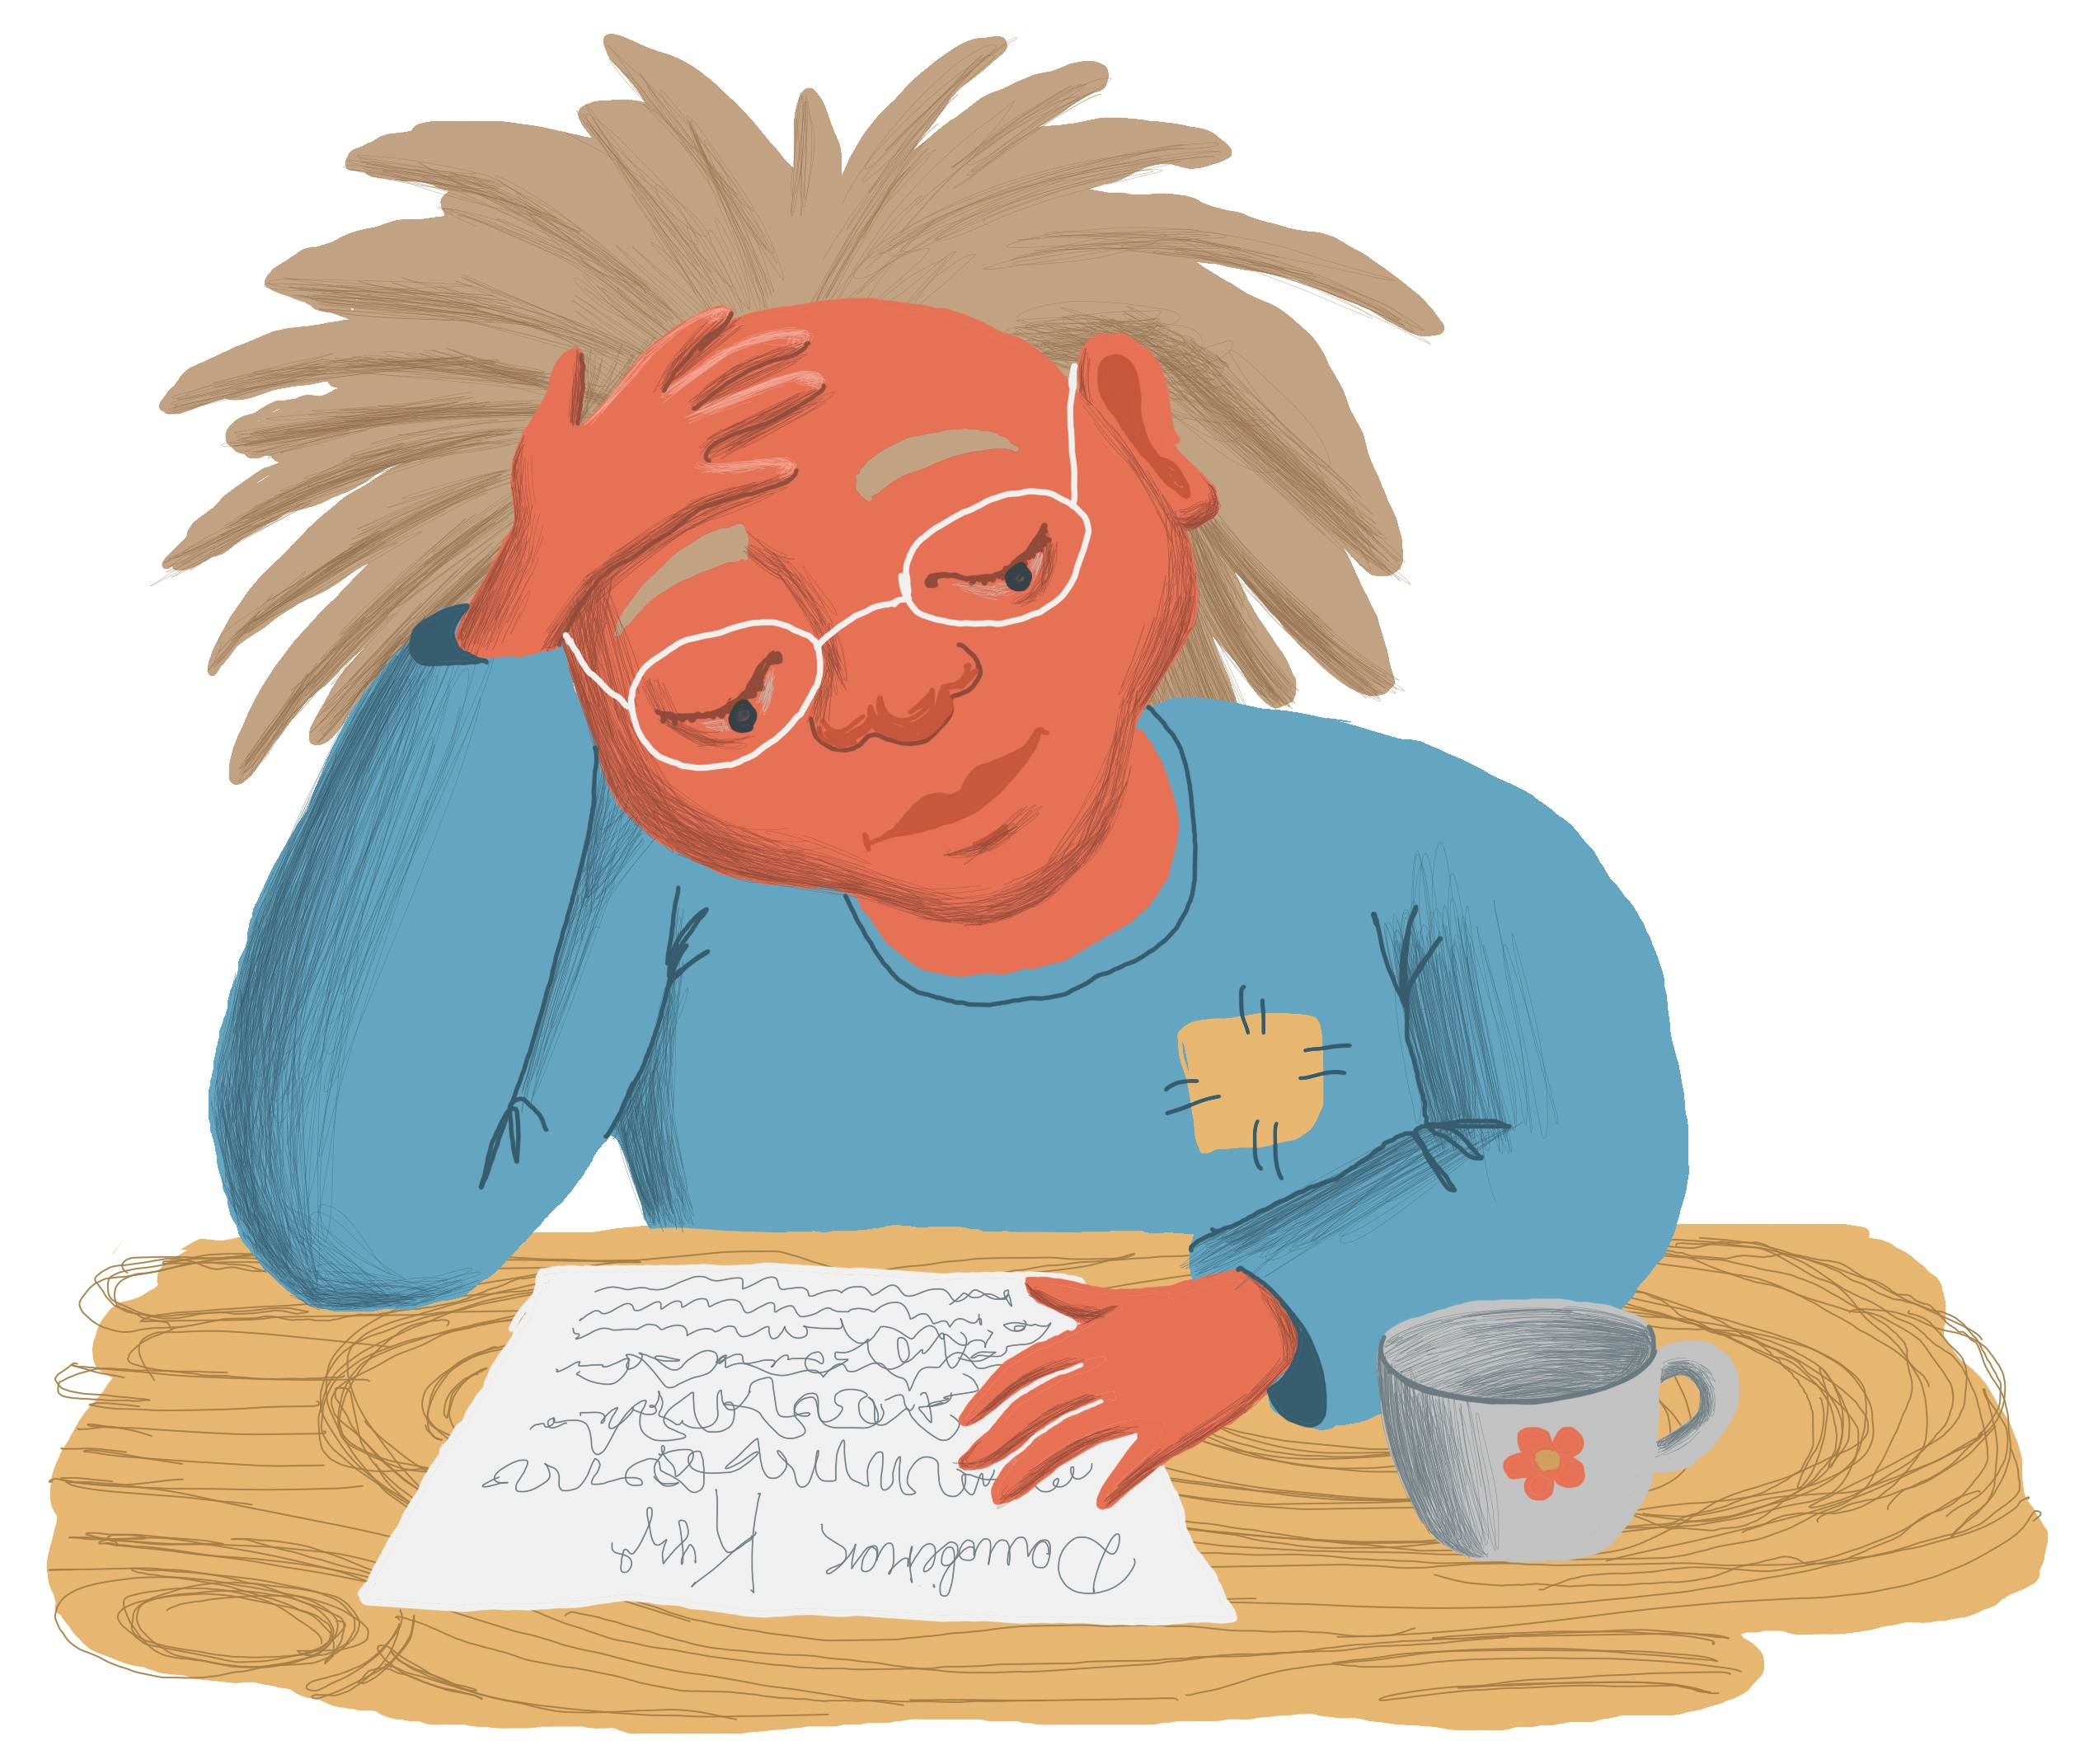
\includegraphics[width=10cm]{figures/color/20c.jpg}
	\vspace{1cm}
	\caption{
             {\itshape Про домовенка Кузю издано 40 статей. 
             Кузя решил заняться их чтением с целью узнать о себе что-нибудь новое }\medskip\\
             \rightline{Задача 1 <<Обаятельный домовенок>>, 2017 год, 4 класс}}
\end{center} \end{figure}

\end{document}